\documentclass{article}

\usepackage[utf8]{inputenc}

\usepackage{parskip}
\usepackage[margin=0.8in]{geometry}
\usepackage{amsmath,amssymb}
\usepackage{amsthm}
\usepackage{bbm}
\usepackage{relsize}
\usepackage{multirow}

\usepackage{graphicx}
\usepackage{wrapfig}

\usepackage{thmtools}
\declaretheoremstyle[%
spaceabove=-3pt,%
spacebelow=12pt,%
headfont=\normalfont\itshape,%
postheadspace=1em,%
qed=\qedsymbol%
]{mystyle} 
\declaretheorem[name={Proof},style=mystyle,unnumbered,
]{prf}
\newtheorem{prop}{Proposition}
\newtheorem{conj}{Conjecture}
\theoremstyle{definition}
\newtheorem{defn}{Definition}

\usepackage[backend=biber]{biblatex}
\addbibresource{prefs.bib}
\usepackage{xcolor}
\definecolor{deepblue}{rgb}{0,0,0.5}
\definecolor{deepred}{rgb}{0.6,0,0}
\definecolor{deepgreen}{rgb}{0,0.5,0}

\usepackage[colorlinks=true, citecolor=deepgreen]{hyperref}
%\usepackage{listings}

\DeclareMathOperator*{\argmax}{arg\,max}
\DeclareMathOperator*{\argmin}{arg\,min}


\usepackage{titlesec}
\titleformat{\subsubsection}[runin]
{\normalfont\bfseries}{--- .{\large\arabic{subsubsection}}}{1em}{}[\mbox{\hspace{0.3em}}]
%{\normalfont\bfseries}{\thesubsubsection}{1em}{}[\mbox{\hspace{1em}}]
\titleformat{\section}[block]
{\normalfont\Large\scshape}{\thesection}{1em}{}

\titlespacing*{\subsubsection}
{0pt}{2.7ex plus 0.7ex minus .2ex}{2.3ex}
\titlespacing*{\section}
{0pt}{7.1ex plus 1.5ex minus .2ex}{3.3ex minus 1ex}

\newcommand{\noised}[2]{\left[#1 \stackrel{\gets}{\sim } #2\right]}

% Python style for highlighting
%\usepackage{courier}


%\DeclareFixedFont{\ttb}{T1}{txtt}{bx}{n}{9} % for bold
%\DeclareFixedFont{\ttm}{T1}{txtt}{m}{n}{9}  % for normal
%
%\newcommand\pythonstyle{\lstset{
%		language=Python,
%		basicstyle=\footnotesize\ttm,
%		breaklines=true
%		otherkeywords={self},             % Add keywords here
%		keywordstyle=\ttb\color{deepblue},
%		emph={MyClass,__init__},          % Custom highlighting
%		emphstyle=\ttb\color{deepred},    % Custom highlighting style
%		stringstyle=\color{deepgreen},
%		frame=,                         % Any extra options here
%		showstringspaces=false            % 
%}}
%\lstnewenvironment{python}[1][]
%{
%	\pythonstyle
%	\lstset{#1}
%}
%{}
%
%% Python for external files
%\newcommand\pythonexternal[2][]{{
%		\pythonstyle
%		\lstinputlisting[#1]{#2}}}

\author{Oliver Richardson (oer5)}
\title{CS6241 Final Project: Doubly Weighted Graph Dynamics and Reddit\\[0.3em]
	\normalsize \url{https://github.com/orichardson/util-graph-dynamics}}
\date{}

\begin{document}
	\maketitle
	
	\section{Introduction}

	
	\subsection{Related Work}
	When formalizing agency, there is a standard assumption that people act to satisfy preferences / utilities which do not change over time --- or at least they ought not to, if the agent is rational. Micro-economists model people in situations where preference changes are not particularly important and time scales are short. At the same time, those interested in machine agency give agents explicit \textit{reward functions} which are part of their identity and have no mechanism for change. 	Humans, however, often do not have well-defined preferences, and change the best-defined ones regularly. 
	The issue of dynamic preferences has recently been an AI safetey concern \cite{amodei2016concrete}, as an agent will likely need to to change more concrete ones as it encounters distributional shift. More directly, the issue has come into focus in certain parts of the philosophy community \cite{grune2009preference}
	
	Meanwhile, there is a standard assumption that graphs are static objects, and often perfectly good temporal structure is thrown out in graph analysis, as recognized by \cite{kostakos2009temporal}\cite{bramsen2006inducing}. However, these formulations of temporal graphs are not obviously continuous, and to my knowledge nobody has done explicitly done the work of thinking of graphs as continuous dynamic objects. Network interpolation based on edit distance \cite{benson19netinterp} is a related problem, but the focus of this paper is not on the functional analysis of graphs as dynamic objects. So far as I can tell, there also has not been much work on discrete choice on static graphs: nodes are not assumed to have "values" per-se, but rather their role is determined purely by their connection to other nodes. In the same spirit might be something like \cite{dugundji2005discrete}, but this imposes a number of other unneeded constraints such as a spatial embedding.
	
	\subsection{This Project}
	Broadly speaking, there are four components to this project, corresponding to sections 2, 3, 5, and 6 ---
	
	\textbf{Section 2: Temporal Graphs.}
	Relatively easy functional analysis aimed at elucidating how we think about temporal graphs, situates them for use with standard functional analysis tools, such as convolutions, and allows you to formulate discrete choice problems in terms of derivatives rather than time steps, which results in qualitatively different behavior.
	
	\textbf{Section 3: Discrete Choice on Graphs.}
	I formalize a few discrete choice models that operate on doubly weighted graphs, show that they result in stochastic matrices, and characterize fixed points.
	
	\textbf{Section 4: Empirical Studies}
	The majority of the effort of the project is the empirical study with reddit data, where I fit my models to a real data set and use some light versions of the theory in the previous two sections to make a bit of sense of the network dynamics
	
	\textbf{Section 5: A Library for Doubly Temporal Graphs.} 
	Finally, in the course of running my experiments, I have produce an artifact of code with many nice properties and some optimized algorithms that my be useful to people in the future looking to do similar kind of work.	
		

	
	\section{Temporal Graph Representations}
	There are many ways of thinking of a graph with temporal information. In class, we saw the formulation presented in \cite{paranjape2017motifs}, in which a temporal graph $T = (V, E)$, where $V$ is a set of vertices (as usual), and $E \subseteq V^2 \times  \mathbb R$ is a collection of time stamped edges. Let $\mathsf{TG}$ be the set of temporal graphs of this kind.
	
	Often people prefer to think of a ``temporalized'' version of a mathematical object $O$ as being a function $\mathbb R \to O$ which gives an object at every point in time. A `temporal graph' of this kind, then, is a graph $G(t) = (V_t, E_t)$ for every time $t$; let $\mathfrak{T}$ be the set of temporal graphs of this kind. If we assume that the vertex set $V_t$ is constant, there are two different ways of embedding the temporal graphs in \cite{paranjape2017motifs}. The first is to simply take the slice $G_{=t}$ of $t$ at time $t$ to be the subgraph which has exactly $t$ as its timestamp.
	
	\begin{align*}
		(-)_{=}&: \mathsf{TG} \to \mathfrak T \\
		&(V, E) \mapsto ~\lambda t.\left( ~V,~\Big\{ (u,v)~\Big|~(u,v,t)\in E \Big\}~\right)
	\end{align*}
	
	Assuming $V_t$ is constant, $(-)_=$ is a bijection, with inverse on edges given by $E \mapsto \{ (u,v,t) \mid \exists t. (u,v) \in E(t) \}$. Of course, this structure is very discontinuous in time, and worse, the set of times $t$ such that the graph slices $E_t$ are inhabited has zero measure. It is reminiscent of a density function. To solve the latter problem, we can integrate over time to get a cumulative graph:
	\[ G_{\leq t} =  \int_0^t (G_{=\tau} )~\mathrm d \tau :=
		 \left( \bigcup_{\tau : [0,t]} V(G_{=\tau}), ~\bigcup_{\tau : [0,t]} E(G_{=\tau}) \right)\]
	
	More explicitly, this gives the following alternate embedding of $\mathsf{TG plus .2ex}$ into $\mathfrak T$:
	\begin{align*}
	(-)_{\leq}&: \mathsf{TG} \to \mathfrak T \\
	&(V, E) \mapsto ~\lambda t.\left( ~V,~\Big\{ (u,v)~\Big|~\exists \tau \leq t.~(u,v,\tau)\in E \Big\}~\right)
	\end{align*}
	
	
	
	\subsection{Weighted Temporal Graphs and Convolution}
	When analyzing temporal graphs, we generally are not interested in the exact times that things happen, but rather we assume that there is some underlying stochastic process that one might like to shed light on. For this reason, we think of the actual data as samples from a stochastic process, rather than the ground truth about what the graph ought to look like.
	
	
	If $G \in \mathfrak T$, then we have an adjacency matrix $A_G(t) : V^2 \to \{0,1\}$ for each time $t$. Continuing our search for continuity, we will add weights to the edges so that $A_G(t) : V^2 \to \mathbb R$ is instead a real-valued function, which can represent partial edges. We can now add, scale, and integrate graphs (with a fixed vertex set) by adding, scaling, or integrating their adjacency matrices.
	%\[ \alpha G + \beta H  = \] 
	Under this interpretation, the integral we wrote earlier may be clearer. We will now show that the representations discussed above can all be expressed in terms of convolutions.
	
	Given a temporal graph $\mathfrak T$ and a kernel function $\phi: \mathbb R \to \mathbb R$, we can define the convolution
	\begin{equation*}
		G \ast \phi := \lambda t.~\int_{\mathbb R}  \phi(t - \tau)(G(\tau))~\mathrm d \tau
	\end{equation*}
	
	In particular,
	\begin{itemize}
		\item 
		 the cumulative graph is a convolution with the Heaviside function $\mathbbm{1}(t) = \begin{cases}
		0 & t < 0 \\ 1 & t \geq 0
		\end{cases}$
		\begin{equation*}
			G_{\leq t} = \int_{-\infty}^t (G_{=\tau} )~\mathrm d \tau  = \int_{\mathbb R} \mathbbm{1}(t - \tau) (G_{=\tau} )~\mathrm d \tau = G_{=} \ast \mathbbm{1} 
		\end{equation*}
		
		\item The windowed graph is a convolution with a window $W_{\pm T}(t) = \begin{cases} 1 & t \in [-T, T]\\ 0 & \text{otherwise}\end{cases}$
		\begin{equation*}
		G_{t \pm T} = \int_{t-T}^{t+T} (G_{=\tau} )~\mathrm d \tau  = \int_{\mathbb R} W(t- \tau) (G_{=\tau} )~\mathrm d \tau = G_{=} \ast W_{\pm T} 
		\end{equation*}	
		
		\item The static graph, obtained by deleting all timing information, can be thought of as a convolution with the constant function $\mathbf 1$:
		\begin{equation*}
			G[:] = \int_{-\infty}^{\infty} (G_{=\tau} )~\mathrm d \tau  = \int_{\mathbb R} 1 \cdot (G_{=\tau} )~\mathrm d \tau = G_{=} \ast \mathbf 1 
		\end{equation*}
	\end{itemize}
	We can also use Gaussian kernels for smoothing, exponential decay, and so forth. One should think of the kernel as the persistence of edges over time.
	
	\subsection{Distance Metrics on Temporal Graphs}
	For non-temporal weighted graphs with the same vertex set, there may be a number of reasonable distance metrics, depending on the application, but since we don't really have a good way to differentiate between edges in the general case, for now we will use the Frobenius norm on adjacency matrices, i.e.,
	\[ d(G,H) = \Big\lVert G - H \Big\rVert_F :=  \Big\lVert A(G) - A(H) \Big\rVert_F = \sum_{u,v \in V} | G_{u,v} - H_{u,v} |^2 \]
	% =\Big\langle G, H \Big\rangle
	
	While this may work well for static graphs, integrating it over time is a terrible idea for dynamic ones --- to see this, let $Q$ be a static weighted graph on a vertex set $V$, $G$ be $Q$ with all edges annotated with a time $t_0$, and $G'$ be $Q$ with all edges annotated with the time $t_0 + \epsilon$, for some vanishingly small $\epsilon$. While $G$ and $G'$ are $\epsilon$-close in some sense (perhaps even the same graph differing by a small timing measurement error), the integrated distance is $2\lVert Q \rVert_F$, and in particular, larger than the distance between $G$ and the trivial 0-weighted graph.
	
	The solution to this is to allow some bleed-over between times: implicitly, we are thinking of time as being somehow persistent. Given some kernel function $k$, we can define a time-smoothed norm on temporal graphs which we can integrate over:	
	\begin{align*}
		\Big\langle -,= \Big\rangle_k: \mathfrak T^2 \to \mathbb R \\
		\Big\langle G, H \Big\rangle_k &:= \int_{\mathbb R}\Big\lVert (A(G) \ast k - A(H) \ast k)(t) \Big\rVert_F~\mathrm d t\\
		&= \int_{\mathbb R} \Big\lVert [(G - H) * k](t) \Big\rVert_F~\mathrm d t 
	\end{align*} 
	
	Note that, while we had motivated this as a distance metric, the final form is only in terms of the difference between the two temporal graphs, making it implicitly a norm. Define $\lVert \cdot \rVert_k : \mathfrak T \to \mathbb R$ by
	
	\begin{equation*}
		\lVert G \rVert_k = \int_{\mathbb R} \Big\lVert [G * k](t) \Big\rVert_F~\mathrm d t 
	\end{equation*}
	\[ \]
	 
	\begin{defn}
		If $T = (V,E) \in \mathsf{TG}$ is a temporal graph and $D$ is a distribution on time offsets, let 
		\[ \noised T D := \left(V,~\Big\{ (u,v,t +d) ~\Big|~ (u,v,t) \in E,~d \sim D \Big\}\right) \]
	\end{defn}
	
	\begin{conj}
		If $k$ is $c$-Lipschitz, $D$ is a distribution with zero mean, and $T \in \mathsf{TG}$ is a temporal graph, then 
		\[ \Pr \left(\left\lVert \noised T {D} _= -~T_= \right\rVert_k \geq \epsilon \right)\leq \frac{c \mathrm{Var}(D)}{\epsilon^2} \]
	\end{conj}
%	\begin{center}
%		\begin{align*}
%			\left\langle \noised T {D} _= -~T_= \right\rangle_k
%				 &= \int_{\mathbb R} \left\lVert \left[\left( \noised T {D} _= - T_=\right) * k\right] (t) \right \rVert_F ~\mathrm d t \\
%				 &= \int_{\mathbb R} \left\lVert \int_{\mathbb R} k(t - \tau)\left( \noised T {D} _{=\tau} - T_{=\tau}\right)~\mathrm d \tau \right \rVert_F ~\mathrm d t\\
%				 &= \int_{\mathbb R} \left\lVert \left(\int_{\mathbb R} k(t - \tau) \noised T {D} _{=\tau} ~\mathrm d \tau\right) - 
%				 \left( \int_{\mathbb R} k(t - \tau)  T_{=\tau}\right) \right \rVert_F ~\mathrm d t\\
%				 &= \cdots
%		\end{align*}
%	\end{center}
	
%	\subsection{The Optimization Problem}
%	
%	This leads us to the following problem: given subspace $\mathfrak S \subseteq \mathfrak T$ of temporal graphs with some desired properties: perhaps smoothness, low number of parameters, etc., and a particular weighted temporal graph $G \in \mathfrak T$, can we find the closest one $H^* \in \mathfrak S$ to $T$?
%	
%	\[ H^* = \arg\min_{H \in \mathfrak S} \Big\lVert H  - G \Big\rVert_k \]
	
	
	\section{Utilities on Graph Nodes} \label{sec:transformer}
	Thus far, we have been considering temporal graphs with edge weights. However, in addition to link strength, we had also wanted to model utilities in the nodes themselves: in our experiments, the nodes will be subreddits, posts, or comments, all of which have some measure of quality for the node itself.
	
%	Accordingly, suppose we have a utility function $U : V \to \mathbb R$ on the nodes of a temporal graph.
	
	\subsection{Simple Logit}
	To begin, let's note what happens in the extremely simple case where the population is modeled by a single chooser, selecting between the nodes of a graph whose edges don't matter. If this chooser has utility $U : V \to \mathbb R$, and we assume noisy selection drawn from a gumble distribution, then we recover a simple softmax of utilities. This distribution is determined purely by intrinsic utility functions of nodes, making choices purely based on the best utility induces a Markov process $P : V^2 \to \mathbb R$ whose transition probabilities are	
	\[ P_{i,j} \propto \exp (U_i - U_j) \]%\frac{\exp(U_u)}{\displaystyle\sum_{v \in V} \exp(U_v)} \]
	
	On the other extreme, if all nodes are equally good, and we just diffuse through the network according to some random walk, perhaps with a Markov process with stochastic matrix $P : V^2 \to \mathbb R$. These could be defined by weighted probability distribution over the weights (if non-negative).
	
	\subsection{Mixing Models}
%	\subsubsection{Stochastic Matrix Mixing}
%	If $P$ and $Q$ are two stochastic matrices defining transition probabilities on $V$, we might want to interpolate between them, mixing some of their properties.
%	Given any function $F : \mathbb R^+ \times \theoremmathbb R^+ \to \mathbb R^+$, we can define a function $\mathrm{Mix}^F_{P,Q} : \mathrm{Stoch}(V) \times \mathrm{Stoch}(V) \to \mathrm{Stoch}(V)$, which creates a new stochastic matrix using $F$ as a scoring function.
%	\[ \Big[\mathrm{Mix}^F_{P,Q}\Big]_{i,j}  \propto~ F( P_{i,j}, Q_{i,j} ) \]
%	
%	Explicitly,
%	\[ \Big[\mathrm{Mix}^F_{P,Q}\Big]_{i,j} = \dfrac{F( P_{i,j}, Q_{i,j} )}{\displaystyle\sum\limits_{v \in V} F( P_{i,v}, Q_{i,v} )} \]
%	
%%	which is defined whenever $F$ is guaranteed to be non-zero .
%	In the case where $F(a,b) = ab$ is just multiplication, and either $P$ or $Q$ comes from a logit model, we have
%	
%	\[ \Big[\mathrm{Mix}^F_{P,Q}\Big]_{i,j} = \cfrac{  e^{u_j} Q_{i,j} }{\displaystyle\sum\limits_{v \in V} e^{u_v} Q_{i,v} } \]
%	
%	
%	\subsubsection{Model I}
	Imagine the following procedure: at node $u$, we draw a non-empty `neighborhood' (which we may or may not require to include $u$ itself) $N_u \subseteq V$ from some distribution depending on the transition probabilities, which favors nodes easy to get to from $u$. From there, we choose an element of $N$ with probability proportional to the softmax of their utilities. This procedure defines a Markov process whose matrix $P$ is given by
	
	\begin{equation}
		P = (u,v) \mapsto \mathlarger{\sum}_{{N \subseteq V}} \left[ \Pr(N; u)~\cfrac{ e^{U_v}  (\mathbbm 1_{v \in V}) }{ \displaystyle \sum\limits_{ s \in N } e^{U_s}  (\mathbbm 1_{v \in N})} \right]
		%\left(\prod_{s \in N}Q_{u,s}\right) \left(~\prod_{s \notin N}(1- Q_{u,s}) )\right)
	\end{equation}
	
	where $\mathbbm 1_{\varphi}$ is an indicator function for the proposition $\varphi$. I have written out the indicator in the bottom sum to more explicitly show that this is (the limit of) a mixed logit model, where the neighborhood $N$ is a latent variable, whose only role is to mask off alternatives that are not observed.
	
	The probability $\Pr(N; u)$ on neighborhoods could be constructed in many reasonable ways --- one could use random walks, even non-Markov ones, to generate paths, and sample from the probability of a given vertex appearing. To analyze the behavior in closed form, we will start by imposing the relatively minor restriction that the neighborhood probabilities depend only on some transition probabilities given by a stochastic matrix $Q$. Re-interpreting the above formula, this gives us a transformer 

	\begin{equation}
		\begin{aligned}
			\Psi&:\mathrm{Stoch}(V) \to \mathrm{Stoch}(V) \\
			\Psi(Q) &:=(u,v) \mapsto \mathlarger{\sum}_{{N \subseteq V}} \left[ \Pr(N; u, Q)~\cfrac{ e^{U_v} (\mathbbm 1_{v \in N})  }{ \displaystyle \sum\limits_{ s \in N } e^{U_s} } \right]
		\end{aligned}
	\end{equation}
	
	A natural question now becomes: when does $\Psi$ have a fixed point? Or equivalently, what are the $\Psi$-stationary stochastic matrices on $V$? In the context of the reddit analysis, such a matrix can be interpreted as an equilibrium flow of attention, where the appropriate attention (aside from some noise) is directed at the highest utility objects
	
	To answer this question, we need to nail down $\Pr(N;u)$ a bit more; the remainder of this section will go through the details for specific neighborhood selection choices.
	
	\subsubsection{$k$-Sample Neighborhoods}
	
	Suppose that our neighborhood is given by $k$ i.i.d. samples from the transition probabilities $Q_{u,-}$ out of node $u$. In this case, $\Pr(N;u,Q) = \prod_{s} Q_{u,s}$ and so our transformer becomes
	
	\begin{equation}
		\Big[\Psi^{(k)}(Q)\Big]_{u,v} := \mathlarger{\sum}_{N \in V^{k}} \left[\left(\prod_{s \in N}Q_{u,s}\right) ~\cfrac{ e^{U_v}  (\mathbbm 1_{v \in N})}{ \displaystyle \sum\limits_{ s \in N } e^{U_s} } \right]
	\end{equation}
	
	First, a few sanity checks: in the specific case where $k = 1$, we get $\Pr(\{j\}; u, Q) = Q_{u,j}$, the transition probability, which is what we had wanted.\\
	
	\begin{prop}
		$\prod_{s \in N}Q_{u,s}$ is a pdf over $N \subseteq V$ of size $k$ , i.e., it is positive and integrates to one.
	\end{prop}
	\begin{prf}
		\begin{align*}
			\sum_{N \in V^{k}}\prod_{s \in N}Q_{u,s} &= 
				\sum_{n_1 \in V} \sum_{n_2 \in V}\cdots \sum_{n_k \in v} \Big(Q_{u,n_1}Q_{u,n_2} \cdots Q_{u,n_k}\Big) \\
				&= \sum_{n_1 \in V} Q_{u,n_1} \Big(\sum_{n_2 \in V}Q_{u,n_2} \Big( \cdots \sum_{n_k \in v} \Big(Q_{u,n_k}\Big)\cdots\Big)\Big) \\
				&= \Big(\sum_{n_2 \in V}Q_{u,n_2} \Big( \cdots \sum_{n_k \in v} \Big(Q_{u,n_k}\Big)\cdots\Big)\Big) \Big(\sum_{n_1 \in V} Q_{u,n_1} \Big)\\
				&\hspace{1in}\vdots\\
				&= \prod_{i=1}^k \Big( \sum_{n_2 \in V}Q_{u,n_i} \Big) \quad
				=\quad \prod_{i=1}^k (1) \quad=\quad 1
		\end{align*}
	\end{prf}

	Next, note that when $k=1$, we aren't actually making any choices, so the decision cannot be influenced by the node utilities; in this case, we recover exactly the distribution $Q$ no matter what the utilities are. More precisely,\\
	theorem
	\begin{prop}
		$\Psi^{(1)}(Q) = Q$
	\end{prop}
	\begin{prf}
		\[ \Psi(Q)_{u,v} = \mathlarger{\sum}_{n \in V} \left[Q_{u,n} ~\cfrac{ e^{U_v}  (\mathbbm 1_{v = n})}{ e^{U_n} }\right] = \sum_{n \in V} Q_{u,n} \mathbbm 1_{v=n} = Q_{u,v} 
		 \]
	\end{prf}

	\begin{prop}
		In general, $\Psi^{(k)}Q = Q$ if and only if, for all $u, v \in V$, \[\displaystyle\mathop{\mathbb E}\limits_{n_1, \cdots n_k \sim (Q_u)^{k-1}} \Big[\mathrm{softmax}(U_{\{v, n_1, \cdots n_{k-1}\}})\Big] = \frac{1}{k}\]
	\end{prop}
	\begin{prf}
		\begin{align*}
			&&Q_{u,v} &= \Big[\Psi^{(k)}(Q)\Big]_{u,v} = \mathlarger{\sum}_{N \in V^{k}} \left[\left(\prod_{s \in N}Q_{u,s}\right) ~\cfrac{ e^{U_v}  (\mathbbm 1_{v \in N})}{ \displaystyle \sum\limits_{ s \in N } e^{U_s} } \right] \\
			&\iff& Q_{u,v} &= k \mathlarger{\sum}_{N \in V^{k-1}} \left[\left(Q_{u,v}\prod_{s \in N}Q_{u,s}\right) ~\cfrac{ e^{U_v} }{ \displaystyle e^{U_v}+\sum\limits_{ s \in N } e^{U_s} } \right] \\
			&\iff& \frac{1}{k} &=\mathlarger{\sum}_{N \in V^{k-1}} \left[\left(\prod_{s \in N}Q_{u,s}\right) ~\cfrac{ e^{U_v} }{ \displaystyle e^{U_v}+\sum\limits_{ s \in N } e^{U_s} } \right] \\
			&& &= \mathop{\mathbb E}\limits_{n_1, \cdots n_k \sim (Q_u)^{k-1}} \Big[\mathrm{softmax}(U_{\{v, n_1, \cdots n_{k-1}\}})\Big]
		\end{align*}
	\end{prf}


	\subsubsection{Independent Inclusion Neighborhoods}
	While the above formulation works out nicely and the probability takes a convenient product form, it also has a hyperparameter $k$. Rather than restricting the size of $N$, we can select each node independently to be part of the choice set with probability $Q_{us}$. This may seem at first glance to be different, but is actually equivalent to a mixture of the above process with binomial coefficients. As a result, really we have not removed any extrinsic choices, but rather marginalized them out with an implicit choice of distribution over the length $k$. In general, for a general distribution $\lambda$ over $\mathbb N$, this means we have a transformer defined as 
	
	\begin{equation*}
		\Big[\Psi^{\lambda}(Q)\Big]_{u,v} := \mathlarger{\mathlarger\sum}_{k \in \mathbb N} \lambda(k) \mathlarger{\sum}_{N \in V^{k}} \left[\left(\prod_{s \in N}Q_{u,s}\right) ~\cfrac{ e^{U_v}  (\mathbbm 1_{v \in N})}{ \displaystyle \sum\limits_{ s \in N } e^{U_s} } \right]
	\end{equation*}
	
	\subsubsection{Binary Choice}
	The complexity of calculating both of the above models is exponential in the highest value of $k$ that contributes a non-negligible probability mass. Therefore, as a final suggestion, we propose the following:
	
	\begin{equation*}
		\Psi(Q;U)_{u,v} = \begin{cases}
			\displaystyle Q_{u,v} ~\frac{\displaystyle 1}{\displaystyle 1 + e^{U_u - U_v}} & i \neq j \\
			\displaystyle Q_{u,u} + \sum_{s: V} \frac{\displaystyle Q_{u,s}}{\displaystyle 1 + e^{U_s - U_u}}& i = j
		\end{cases}
	\end{equation*}
	

	
%	However, one might not have knowledge of all of the nodes, but instead only samples of utilities from a small neighborhood of them. One datamight have various ways to get from one node to another, determined by transition probabilities, $P_{i,j}$
	

	
	\section{Doubly Weighted Temporal Graphs}
	We would ultimately like to develop theory for graphs which have both vertex and edge weightings which vary over time. If $G \in \mathfrak T$ is a temporal graph, we would like to use utilities $U : V \to E$ to explain changes in the graph weights over time.  This corresponds to finding a solution to the optimization problem
	
	\[ \Xi^* = \arg\min_{\Xi} \Big\lVert \frac{\partial G}{\partial t} - \Xi(G;U)  \Big\rVert_\phi \]
	
	for some persistence kernel $\phi$, where $\Xi: \mathfrak T \times R^{V(\mathfrak T)}$ ranges over graph transformers such as the ones in section \ref{sec:transformer}.
	
	\section{Experiments}
	The second, and primary branch of this project is an empirical one: we focus on the task of predicting the future connectivity of a temporal graph based on its current configuration, including both vertex and edge weights. Rather than predicting the raw weights from these temporal graphs, we first column-normalize them, for several reasons:
	
	\begin{enumerate}
		\item As with with many real world data-sets distribution of most connectivity metrics (number of links included) across sub-reddits is heavy-tailed and unbounded. Moreover, the problem is worse for temporal graphs: there may not be temporal consistency in the weightings. For instance, Reddit as a whole is still growing, and so any method trained on the past would be off-distribution for the future in terms of raw magnitude.
		
		\item Many of the simple methods at our disposal are very scale sensitive, and often explicitly expect zero-centered and unit-variance. SVM's are notorious for requiring a great deal of pre-processing to get good results.
		
%		\item It makes the discrete choice methods above 
		
		\item It is still enough information to understand the dynamics of a graph: the column-normalized adjacency matrix $Q$ of a graph $G$ is enough to totally determine a linear markov process on the weights, which means that $Q$ is sufficient to construct most centrality and role-labeling methods, such as page-rank vectors, node2vec embeddings, and so forth.
		
	\end{enumerate}
	
	The net effect of this is to give all of the methods below a boost, by allowing them to predict an easier problem, focused on the relative connectivities of the nodes, rather than the absolute scale of the values, which is less interesting from our perspective. With this in mind, our precise research question we target is as follows:
	
	\textbf{Research Question:} \textit{ Given a stochastic transition matrix $Q_t$, arising from the column-normalized weight matrix of a the graph a time $t$, can we use the discrete choice models discussed above to predict the transition matrix at time $Q_{t + \Delta T}$ at some future time $t + \Delta T$? }
	
	
	\subsection{Data}
	For the experiments which follow, we view Reddit as a doubly weighted temporal graph, in which the nodes are subreddits, and the edges are numbers of links between them posted at a given time, i.e., in subreddit \texttt{r/A} a user might post a comment containing the string \texttt{r/B}. To someone who hasn't interacted with the site much, such links may  not seem like a very strong signal, but in fact posting one is an incredibly common contribution, and can carry a great deal of information: it is often used as a concise way of pointing to a particular, well-known trope. For instance, people who fail to recognize a joke might be referred to \texttt{r/wooosh}, an arrogant submission might be referred to \texttt{r/iamverysmart}, and a mean-spirited one to are\texttt{r/trashy}. 
	
	The fact that people often don't know about these communities (some of which are better than others) and follow them, or re-discover them by seeing references, rather than simply scrolling through an algorithmically determined feed, makes Reddit a place particularly suited to this kind of network.
	
	\subsubsection{Formal Graph Description} \label{sec:formalmodel}
	
	Because Reddit contains a lot of data across a giant period of time in a lot of different places, my data does not consist just of a single temporal graph, but rather many subgraphs of different numbers of nodes, across different time windows, and with varying temporal precision.
	
	For a time interval $T$, a threshold paramter $\theta$, and size parameter $N$, I form a temporal subgraph with a fixed number of nodes, by identifying the $N$-highest utility nodes, call them $V_N$, and setting, for each $u,v \in V_N$ and $t \in T$,
	\begin{align*}
		(W_{u,v})_t &= \text{\# links u$\to$v posted at time $t$} \\
%		Q_{u,v}_t &= \frac{W_{u,v}_t}{\displaymode \sum_{s} W_{u,s}_t } \\
		(U_{u})_t &= \text{\# of posts with $\theta$ or more comments in u posted at time $t$}
	\end{align*}
	Because it is faster and more efficient to do this with a smaller number of discrete items in $T$, we model time as a number of discrete windows. We arbitrarily choose $\theta = 9$ to exclude posts with very few comments. 
	
	\subsection{Predictors}
	In addition to our own models, we run a battery of additional baselines.
	
	\subsubsection{Constant Function.} The easiest thing to do (which turns out to be very difficult to beat), is to predict that the transition matrix does not change, i.e., predict $Q_{t+\Delta T} = Q$. The effectiveness of this model points to the difficulty of the task.
	
	\subsubsection{Random Noise.} An even worse baseline is a random matrix (elements drawn iid from a uniform distribution), scaled to be stochastic (each column summing to 1). While there is no shame in failing to beat the constant function (after all, conservatism is very safe and quite effective!), this baseline is the performance floor.
	
	\subsubsection{The Identity Matrix.} The prediction $Q_{t+\Delta T} = I$ corresponds to users only referencing the sub that they're currently posting in, oblivious to the rest of the website.
	
	\subsubsection{Matrix Powers.} \label{sec:matrixpowers} Here we predict $Q_{t+\Delta T} = Q^{n}$ for some $n \in \mathbb N$. This corresponds to paths of exactly $n$ hops along a random walk given by $Q$. If Reddit users were ignoring content and merely clicking on every sub link, then posting a submission or comment, we would expect the evolution of the graph to look like this, and for $Q$ to be a fixed point of itself if the dynamics were stable.
	
	Note that this subsumes the constant function and identity matrix baselines, with $(n=1)$ and $(n=0)$, respectively. Because of our interpolation methods (below), we will also see data for fractional powers of matrices, so we will get the entire spectrum between the two.
	
	\subsubsection{SVMs.}
	We now use some more sophisticated baselines. We use support vector machines (SVMs) with linear and rbf kernels as regressors from the entire transition matrix, to each individual matrix element. If it were the case that this prediction problem was totally different for each subreddit identity, we would expect a method like this (although perhaps with a more sophisticated, kernel, such as one corresponding to a deep net) to outperform everything else, given enough training data.
	
	\subsubsection{Linear Models.}
	We also use linear least squares in two ways: first, in the same way that we train the SVM's above: predicting each matrix element of $Q_{t + \Delta T}$ independently, and a second, we estimate $A \in \mathbb{R}^{|Q|^2 \times |Q|^2}$ directly using a single application of linear least squares on the entire dataset.
	
	\subsubsection{Inversion Averages} We can also naively average the linear transformations seen in the training set to estimate what a matrix linear transform might look like:
	\[ Q \mapsto \left(\frac{1}{T}\sum_{t = 1}^T Q_{i+1} (Q_i)^{-1} \right)Q \]
	In practice, some matrices are only barely invertable, so as written, this method generates a matrix with entries of giant magnitude. To prevent this from hugely skewing averages, we clamp the values of the inverted matrix to $[-1,1]$,  
	
	\subsubsection{Discrete Transformers} Finally, we arrive at the methods developed in the previous section. We make some use of $\Psi^{(k)}$ for $k= 2,3$, and mostly focus on the non-subscripecause Reddit contains a lot of data across a giant period of time in a lot of different places, my data does not consist just of a single temported one $\Psi$, because it performs similarly (or better) empirically, and is much faster to compute, as $\Psi^{(k)}$ takes time exponential in $k$ to calculate without approximation.
	
	\subsection{Covariates and Parameters}
	\subsubsection{Interpolation} 
	Because our methods are discrete in nature, we need a way of making their impact smaller when less time has elapsed. To this end, we form an $\alpha$-mixture with the constant function to obtain our final result. More explicitly, given a predictor $f$, which takes as arguments a matrix $Q$ and perhaps other arguments such as utilities $(-)$, we instead use one of the functions below as our predictor for $Q_{t + \Delta T}$:
	\[\text{Linear: } (Q, -) \mapsto (1-\alpha) Q + \alpha f(Q,-) \qquad\qquad 
		\text{Multiplicative: } (Q,-) \mapsto \Big(f(Q,-)Q^{-1}\Big)^\alpha Q \]
	
	\subsubsection{Temporal Offset}
	In principle, we could also fix the above problem by explicitly setting up the learning task by tailoring the temporal offset $\Delta T$ explicitly to our discrete choice methods. This is in some sense the dual to changing the interpolation parameter, except it also impacts the performance of the other predictors, which are actually fit to data. The way that this plays out (especially with respect to the mixture coefficient $\alpha$) is one of the more interesting results below.
	
	\subsubsection{Graph Characteristics}
	As described in section \ref{sec:formalmodel}, I have many different temporal subgraphs of Reddit data that I have trained on, whith different paramters, such as numbers of nodes, time windows, and temporal precision. Some of these characteristics, in particular, the number of nodes in the graph, have an important, non-trivial role to play in the the difficulty of the learning problem. 
	
	\subsubsection{Utility Scaling}
	Finally, because logit models are not scale-free in utility, the scaling of the utility metric matters. Because my surrogate for ``utility'' has numbers on the order of $10^7$ for some nodes and $10^2$ for others, taking the exponential of the difference between these numbers is rather ridiculous. I have three modes of dealing with this problem:
	\begin{enumerate}
		\item Take $U = \log U$, which undoes this exponential distribution, and effectively turns the logit model into a normal weighted coin. This is a reasonable thing to do if you think that the number of posts in a subreddit is already the exponential of some internal utility
		\item Scale $U$ so that its maximum value is a constant, $\mathsf U_{\text{max}}$. This preserves the logit flavor of the model. As $\mathsf U_{\text{max}}$ goes to zero, the discrete choice models approach diffusion, as everything has the same utility. Accounting for this implicitly gives us one more baseline: the laplacian matrix $LQ$
		\item Simply divide utilities by a big constant so it's possible to compute with them. This leaves the absolute magnitude in the equation somehow, but there is no principled way of setting factor you divide by.
	\end{enumerate}
	
	
	\section{Results and Discussion}
	Each heading below is a non-trivial result.  As this is an exploratory study, I have looked at my data from many different angles. Combined with the fact that there is not a clear way to measure the number of degrees of freedom for many of the quantities I measure, it would be misleading to report $p$-values. Nonetheless, each finding I report persists across different slices of the reddit graph, and is stable, as far as I can tell---I have explicitly tried to falsify all of them. In some cases, I illustrate this with multiple figures, tables, or averages, but in general there is not enough space to include all of the evidence. 
	
	Although I believe all of these trends hold, a more targetted study would be required in order to fully establish any of the claims I make here. In an effort to make sense of the data, I also include some post-facto speculation in which I retroactively guess the causes for trends; this, too (and perhaps especially), should be taken with a grain of salt. 
	
	On that note, let's start with a depressingly negative result:	
	
	\subsection{Without Interpolation, The Constant Function Outperforms Everything}\label{sec:godconst}
	This is true across all graph slices. Consider figure \ref{fig:constgood}. On the left, we have $Q^2$, and the right, $Q$, used as predictors for $Q$ at a different time step. The $Q_t$ used to produce the prediction is on the right, and the prediction target time is given by the x-axis. This visualization is cluttered but lets us verify that there is nothing special going on temporally that would cause an average to hide things (for instance, if the graph didn't change throughout the year of 2018, causing the constant predictor to be better on average).
	
	\begin{figure}[h]
		\centering
		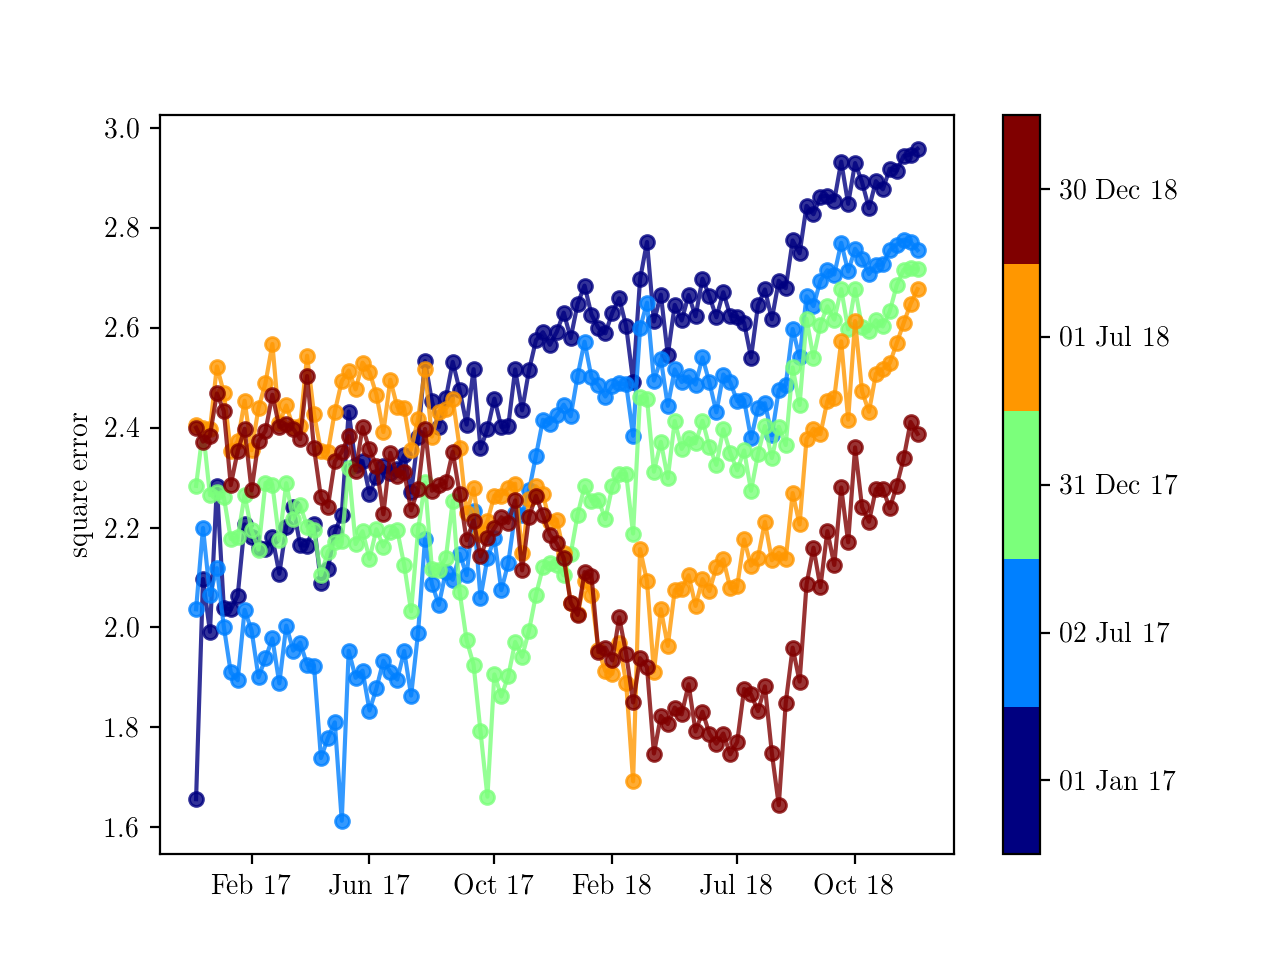
\includegraphics[width=0.49\linewidth]{figs/t_vs_err/Q2}
		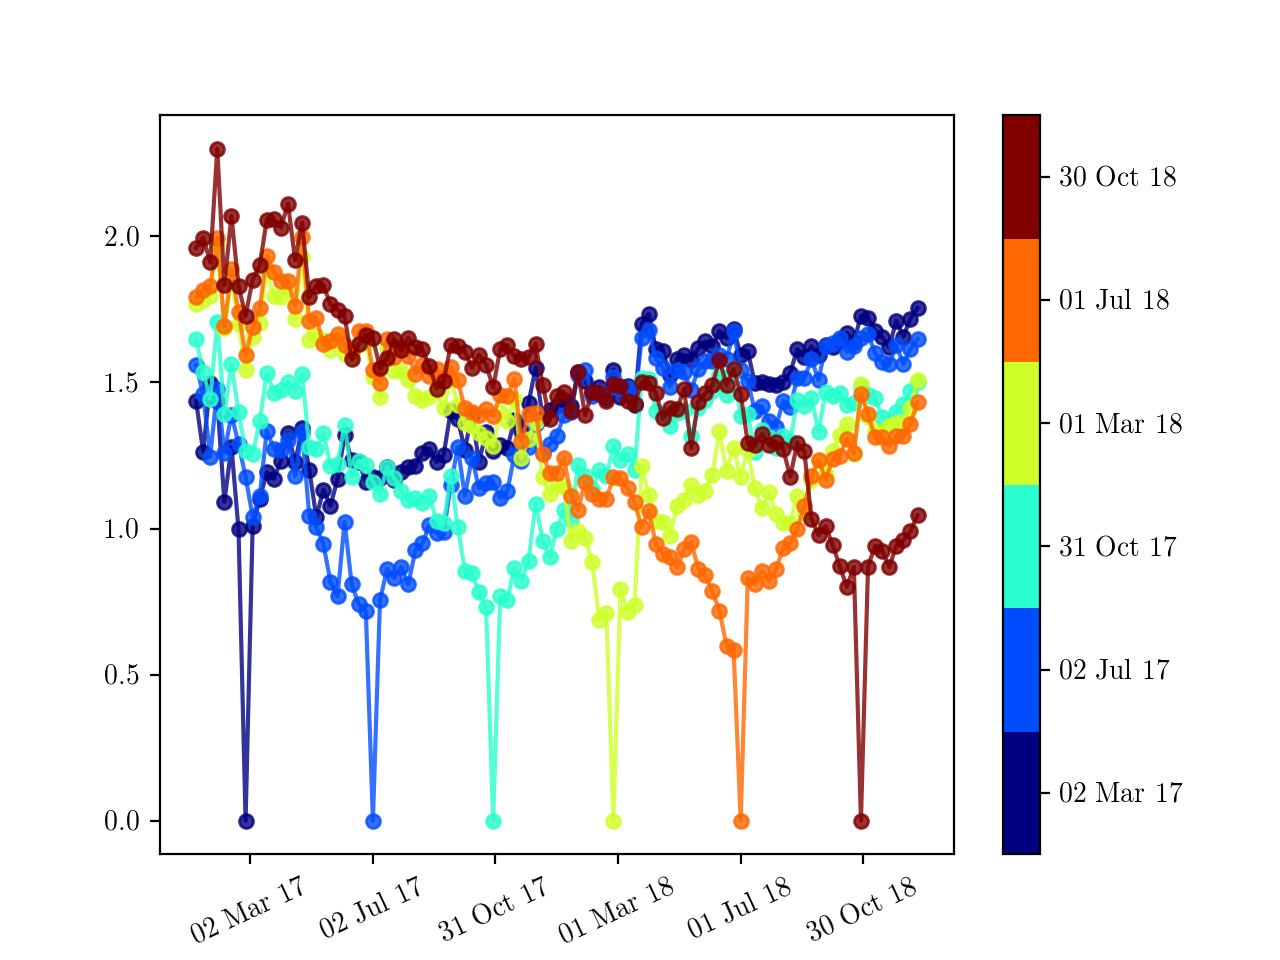
\includegraphics[width=0.49\linewidth]{figs/t_vs_err/Q_id}
		\caption{\color{darkgray} Errors for $Q_n^2$ (left) and $Q_n$ (right) as predictors for $Q_t$. $n$ is chosen based on the bar to the right, and $t$ is the x-axis}\label{fig:constgood}
	\end{figure}
	
	While our binary choice method, $\Psi$, outperforms $Q^2$, it does not even come close to the constant predictor, as seen in figure \ref{fig:static_v_choice}, where they are overlaid. These data are all from the 100-node temporal graph of most active subreddits from 2017-2019, but this is definitely the most robust feature of the data-set. There does not exist a time span $\Delta T$ for which $\Vert\Psi Q_t - Q_{t + \Delta T}\Vert > \Vert Q_t - Q_{t + \Delta T}\Vert$.
	
		
	\begin{figure}[h!]
		\centering
		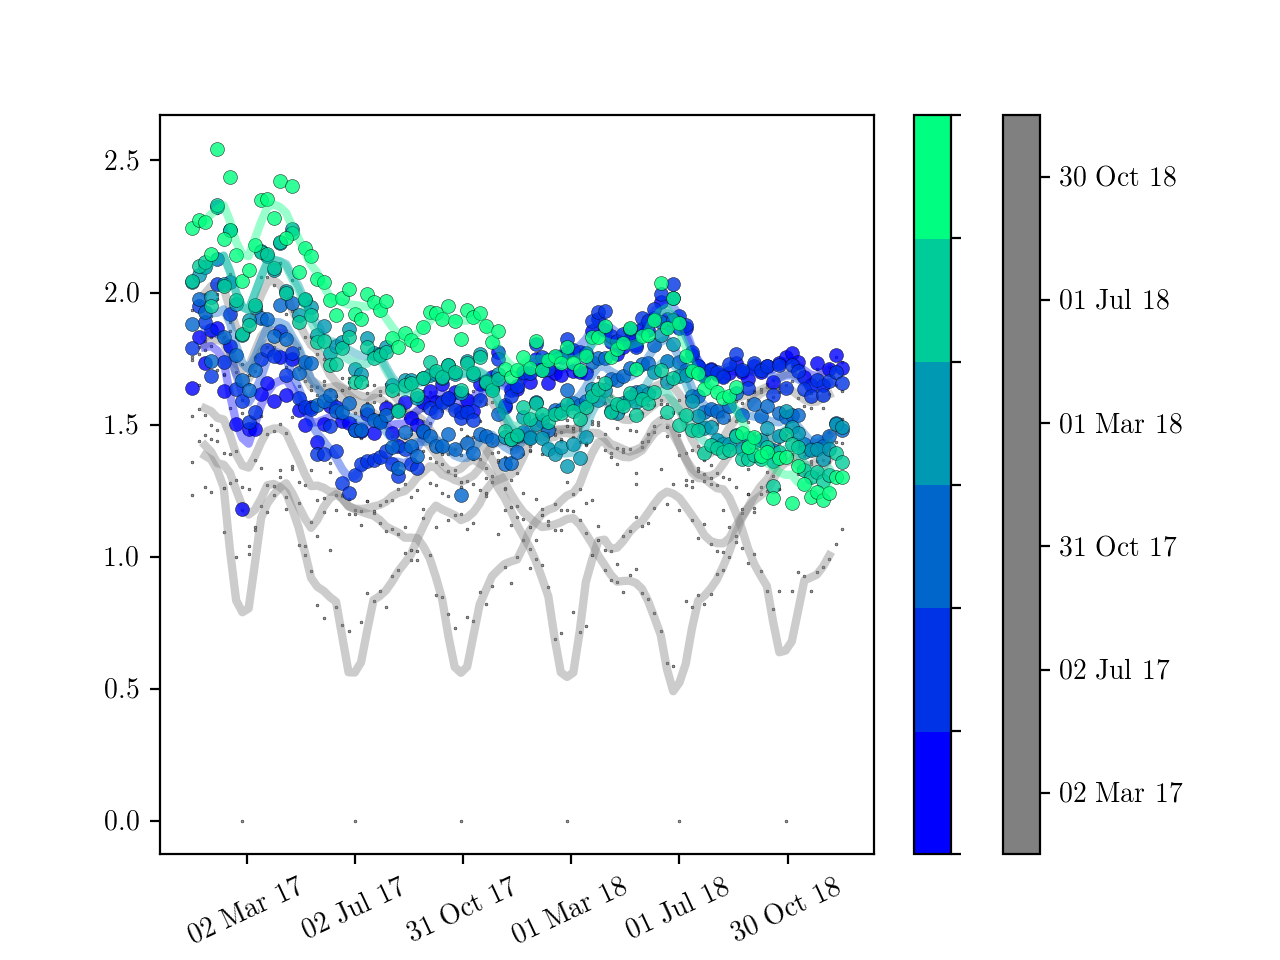
\includegraphics[width=0.7\linewidth]{figs/t_vs_err/choice_vs_static2.png}
		\caption{\color{darkgray} Errors for $\Psi$, in color, and the constant predictor $Q$, in gray. The different trends lines correspond to samples of $Q_t$ used to make the prediction, taken from different times.} \label{fig:static_v_choice}
	\end{figure}

	\clearpage
	\subsection{Higher Matrix Powers are Really Bad}
	
	\begin{wrapfigure}[7]{l}{0.3\textwidth}
		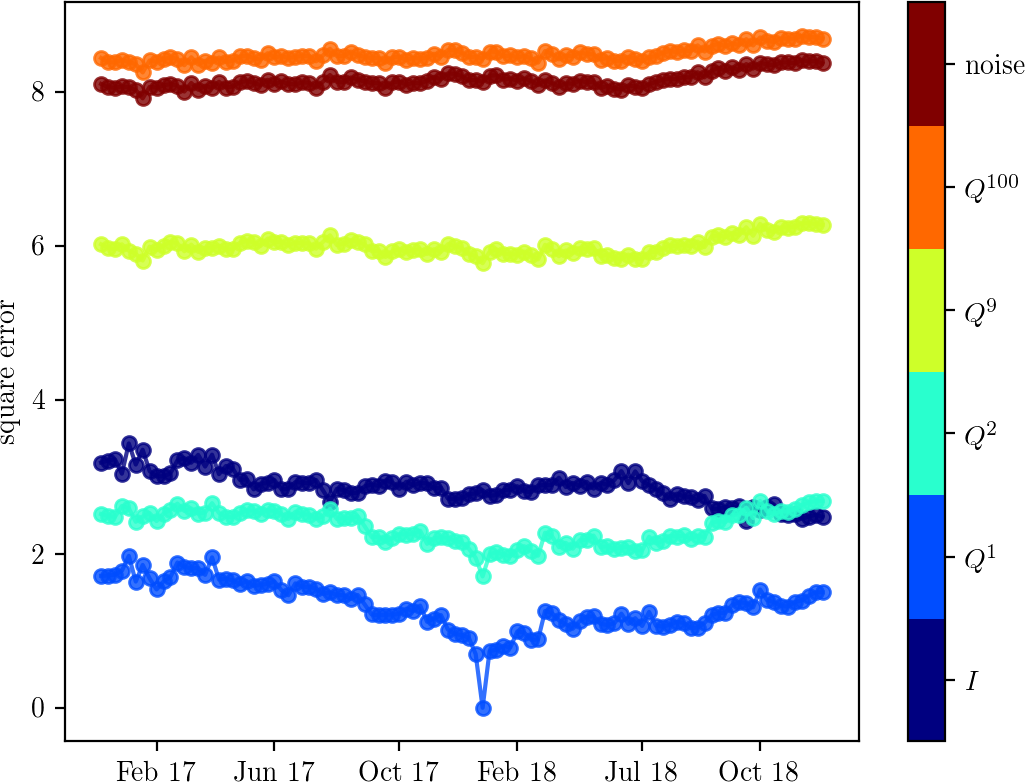
\includegraphics[width=\linewidth]{figs/t_vs_err/Q_powers_limit.png}
	\end{wrapfigure}
	Because the visualization before is so cluttered, we'll throw out everything but the middle point, and look only at the matrix powers in figure \ref{fig:matrix_powers}. Note that each matrix power is strictly worse than the previous one, independent of what it is being used to predict. This goes against the prediction we made in section \ref{sec:matrixpowers}, where we speculated that $Q$ might be its own fixed point due to local stability. The limit point is approached by $Q^{100}$, on the right graph, which is even worse than everything else.
	
	\begin{figure}[h!]
		\centering
		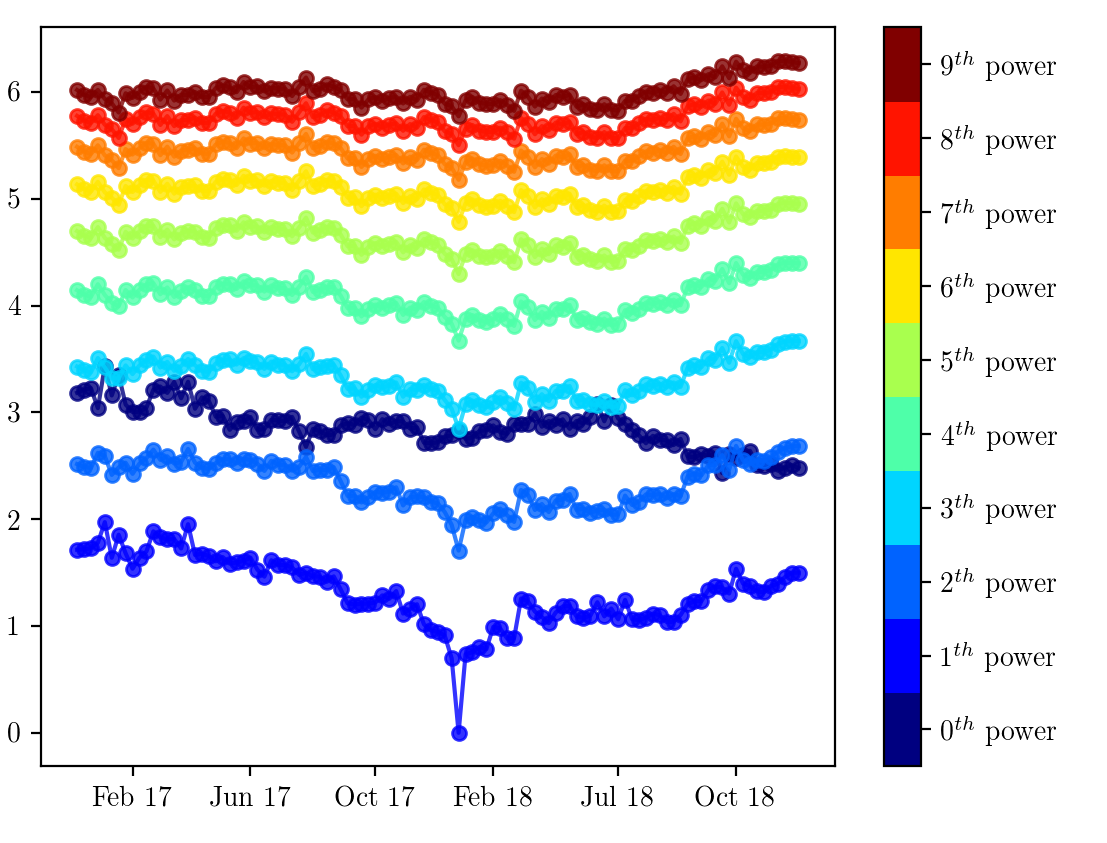
\includegraphics[width=0.52\linewidth]{figs/t_vs_err/Q_powers_halfway_all_cropped.png}
		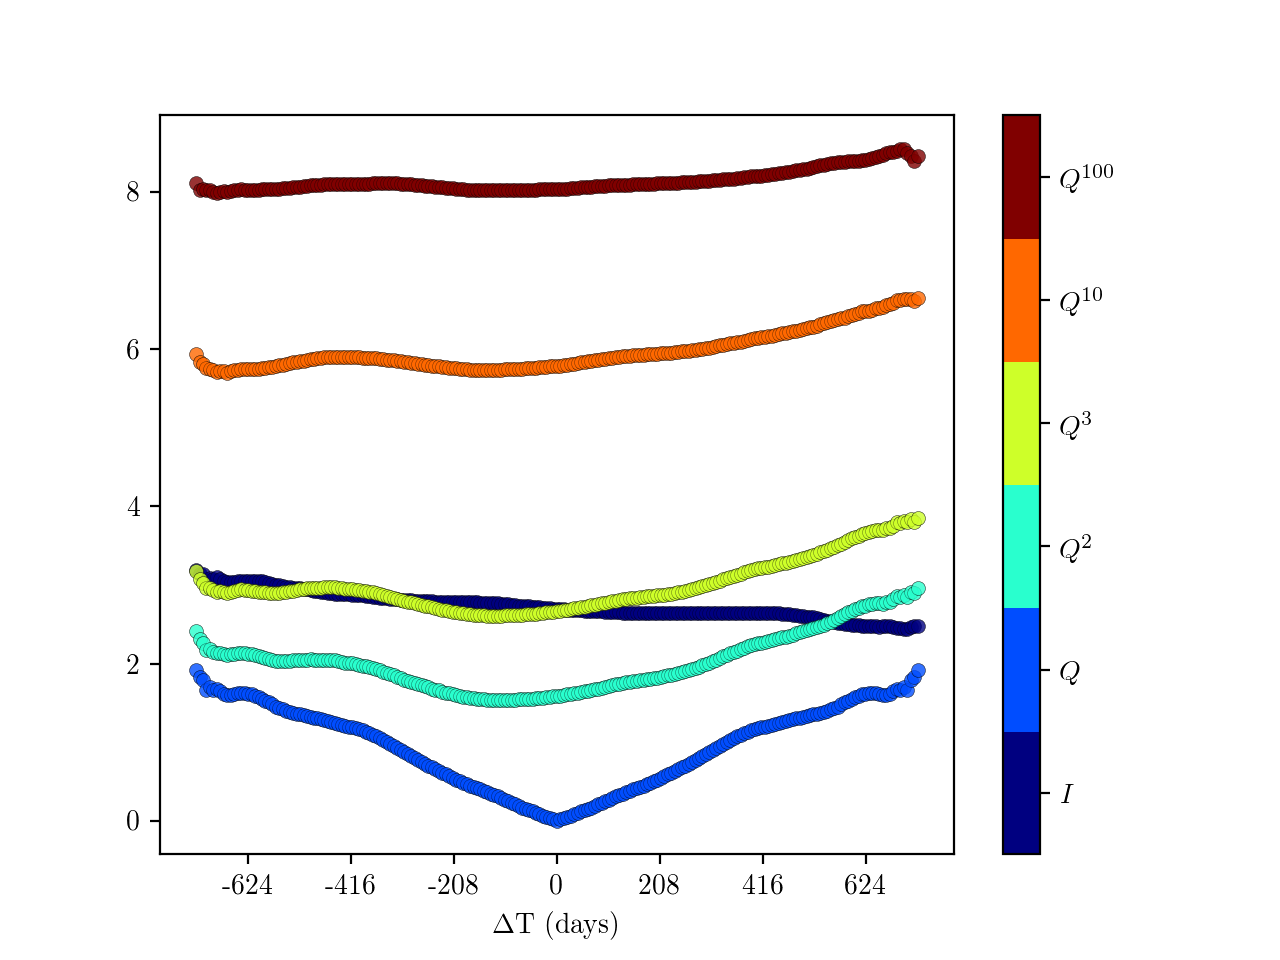
\includegraphics[width=0.47\linewidth]{figs/dt_vs_err/Q_powers_no_conv.png}
		\caption{\color{darkgray} Matrix Power Errors. Left: for 100 nodes, single sample. Right: for a 30-node graph section, averaged across time deltas for stability} \label{fig:matrix_powers}
	\end{figure}

	
	
	By the time that the matrix exponents get above 7, in this case, matrix powers are even worse than normalized noise, as seen on the left.
	

	Another strange feature of both of these is that the identity matrix becomes a better predictor over time. This lends credibility to our next finding:
	
	
	\subsection{Reddit is Slowly Moving Towards Subreddit Isolation}
	
	Look again at figure \ref{fig:matrix_powers}. Note that, even averaged across all time steps, the identity function shows a very clear negative slope. This must mean that, no matter where you anchor your prediction, predicting the identity function is worse if you look at previous times than if you look at future ones --- and therefore, as time goes on, more and more references to a subreddit are posted inside itself.
	
	\subsection{With the Right Interpolation, $\Psi$ Outperforms Everything}
	
	Now, for the good news: by adding interpolation, $\Psi$ outperforms every other model, including the fancier trained ones, despite having only a single parameter ($\alpha$), rather than a huge collection of support vectors or giant weight matrices. Now, this difference is very small, but but definitely significant, as it persists not only across graphs, but also across utility scalings. In table \ref{tab:full}, you can see the results for most of the baselines that we have not yet seen on one particular graph. 
	
	\begin{table}
		\centering

		\begin{tabular}{cccc}
			& Square Error & Name & $U$-scale \\\hline
			\multirow{16}{*}{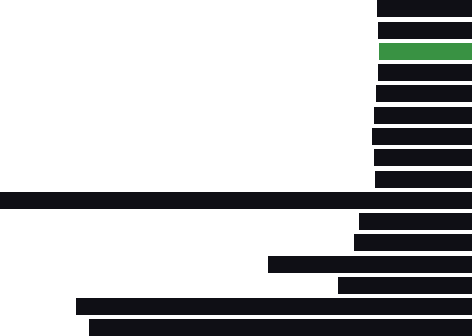
\includegraphics[width=1cm,height=19em]{figs/bar}}
			& 0.000361 & $\Psi_{\alpha=0.06+}$ &\texttt{norm10} \\
			&0.000355 & $\Psi Q_{\alpha=0.13+}$ & \texttt{norm10} \\
			&0.000354 & $\Psi Q_{\alpha=0.2+}$ & \texttt{norm10} \\
			&0.000355 & $\Psi Q_{\alpha=0.25+}$ & \texttt{norm10} \\
			&0.000363 & $\Psi Q_{\alpha=0.35+}$ & \texttt{norm10} \\
			&0.000373 & $\Psi^{(2)} Q_{\alpha=0.1+}$ & \texttt{norm10} \\
			&0.000379 & $\Psi^{(2)} Q_{\alpha=0.2+}$ & \texttt{norm10} \\
			&0.000373 & $\Psi^{(3)} Q_{\alpha=0.1+}$ & \texttt{norm10} \\
			&0.000368 & $Q$ & --- \\
			&0.001791 & AvgInv & --- \\
			&0.000426 & SGDRegressor & \texttt{norm10} \\
			&0.000445 & SGDRegressor & No $U$ provided \\
			&0.000775 & LinearSVR & \texttt{norm10} \\
			&0.000509 & LinearSVR & No $U$ provided \\
			&0.001453 & rbf SVR & \texttt{norm10} \\
			&0.001500 & rbf SVR & No $U$ provided \\
		\end{tabular}
		\caption{\color{darkgray} Errors across predictors, $\Delta T = $ 4 days, $|G|$ = 30 Nodes, 2013-2015}\label{tab:full}
	\end{table}

	There are a number of things to notice here: first, the margin by which our model beats the constant predictor is very slim. However, the difference cannot be attributed to noise, as we will see in later on (for instance, in fig \ref{fig:nnodes_bias_dir}, you can clearly see how much better $\Psi$ for future predictions than past ones) ---- not only clearly persists across a number of graphs.
	
	More things to note: linear SGD and the rbf SVR both benefit from the utility information. This is true for the other graph I ran as well. However, Linear SVR does not benefit from this, and it's not clear why this is the case. More experiments would be necessary to identify why this is happening, but unfortunately, the linear SVR actually takes the longest to train of any of these models. In the end, this probably does not matter, because all of the support vector machines are actually quite bad predictors. The average inversion is also a terrible predictor, which surprised me, but makes some sense because we're averaging in the wrong space.
	
	More extensive tabular results are pre-computed and availble in raw text form at \url{https://github.com/orichardson/util-graph-dynamics/blob/master/writing/raw\_results.txt}, which validate the the claims I'm making further, but to save space, and save myself the trouble of typsetting tables, I will leave the rest of them there.
	
	
	\subsection{Linear and Multiplicative Interpolation are Very Similar}
	
	
	\begin{wrapfigure}{r}{0.3\linewidth}
		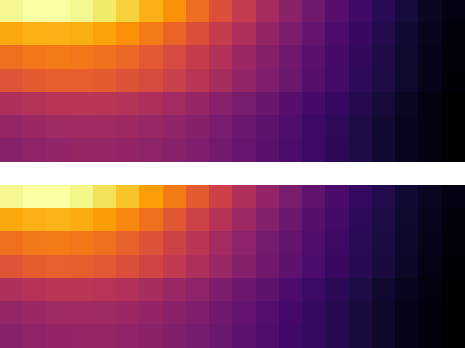
\includegraphics[width=\linewidth]{figs/heatmaps/t_mult,t_lin.png}
		\caption{\color{darkgray} Linear and Multiplicative Mixtures, error on $\alpha \times \Delta T$}
		\label{fig:multadd}
	\end{wrapfigure}
	This is most visually convincing from a heat map: see figure \ref{fig:multadd} on the right. There are two stacked heatmaps: in each, the color represents error (brighter is smaller), going right represents a higher value of $\alpha$ (which ranges from 0 to 1, so in particular, the left side of both diagrams is just the constant predictor $Q$), and going down represents a higher value of $\Delta T$. 	
	To get a clearer visualization of similar error colors, we are actually plotting 
	\[ \frac{1}{10^{-15} + E} \]
	The upper heat map is multiplicative interpolation, and the lower one is additive interpolation. Not only are they visually indiscernable, we also have numbers, in table \ref{tab:multadd}. 

	
	\begin{table}[h!]
		\centering
		
		\begin{tabular}{c|cc}
			 Square Error & $\alpha$ & Interpolation Method \\\hline
			0.00006581 & 0.06 & Linear \\
			0.00006625 & 0.06 & Multiplicative\\
			0.00006608 & 0.04 & Linear \\
			0.00006641 & 0.04 & Multiplicative \\
			0.00006577 & 0.11 & Linear \\
			0.00006629 & 0.11 & Multiplicative \\
			0.00006703 & 0	& --
		\end{tabular}
		\caption{Errors across predictors, $\Delta T = $ 4 days, $|G|$ = 100 Nodes, 2017-2018}\label{tab:multadd}
	\end{table}
	
	The things to take from this table are: (1) linear and multiplicative interpolation result in very similar errors, (2) multiplicative is consistently slightly worse than additive, and (3) all of these again beat the constant predictor, again by a very small margin. 
	

	
	\subsection{Fractional Matrix Powers Don't Help}
	While interpolation helps for our methods, they still do not help the matrix powers. In figure \ref{fig:fracmat} are heatmaps of the same kind as before. The bottom one is the same as in figure \ref{fig:multadd}, and the top one is the equivalent heatmap for the $Q^2$ predictor. 
	
	
	\begin{wrapfigure}[8]{L}{0.3\textwidth}
		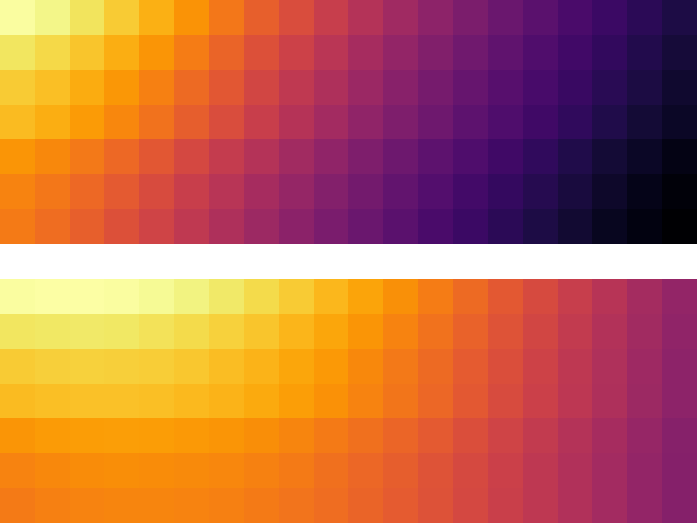
\includegraphics[width=\linewidth]{figs/heatmaps/multiiplicative_interp_Q,Q2,trans_alt.png}
		\caption{\color{darkgray} Fractional powers of $Q^2$ (top), and of $\Psi Q$ (bottom).}
		\label{fig:fracmat}
	\end{wrapfigure}
	The feature of importance is that the $Q^2$ predictor's heatmap is monotonically increasing in error, both in $\alpha$ and in $\Delta T$. Multiplicative interpolation from $Q$ to $Q^2$ corresponds to fractional powers of $Q$, so this means that at no fractional point does a mixture of $Q^2$ and $Q$ outperform $Q$ alone. This is also anecdotally true for linear mixtures, but not shown.
		 
	

	This monotonicity is notably NOT shared by $\Psi Q$, whose brightest squares are not directly on the left edge, but rather a few further right. Once again, we remark that this is another instance of $\Psi Q$ achieving lower error than $Q$. 
	

	\vspace{1in}
	
%	\subsection{Very Small Values of $\alpha$ do not Improve Performance}
	\subsection{Number of Nodes Dictates Forward/Backward Bias of $\Psi$}\label{sec:futurebias}
	
	In my view, the following is the most interesting result: for temporal graph slices that include a large number of nodes (and therefore, some with lower post activity), the accuracy of $\Psi Q$ looks like a future shifted version of $Q$\footnote{Remember that $\alpha = 0$ corresponds to the constant function $Q$, in dark blue}, plus some additional error. See, for instance, the bottom row of figure \ref{fig:nnodes_bias_dir}. This is a really pretty result. Combined with our negative result in section \ref{sec:godconst}, this suggests that we are indeed approximating a partial derivative 
	\[\Psi Q \approxeq \frac{\partial Q}{\partial T} \]
	as opposed to merely sampling the function at some point in the future.
	
	Now for the weirder bit: now take a look at the top line of figure \ref{fig:nnodes_bias_dir}. Here we see a similar (but less pronounced) shift backwards in time. Evidently, for $N=9$, $\Psi Q$ predicts the past better than it predicts the future.
		
	\begin{figure}
		\centering
		\vspace{-3em}
		($N=9$)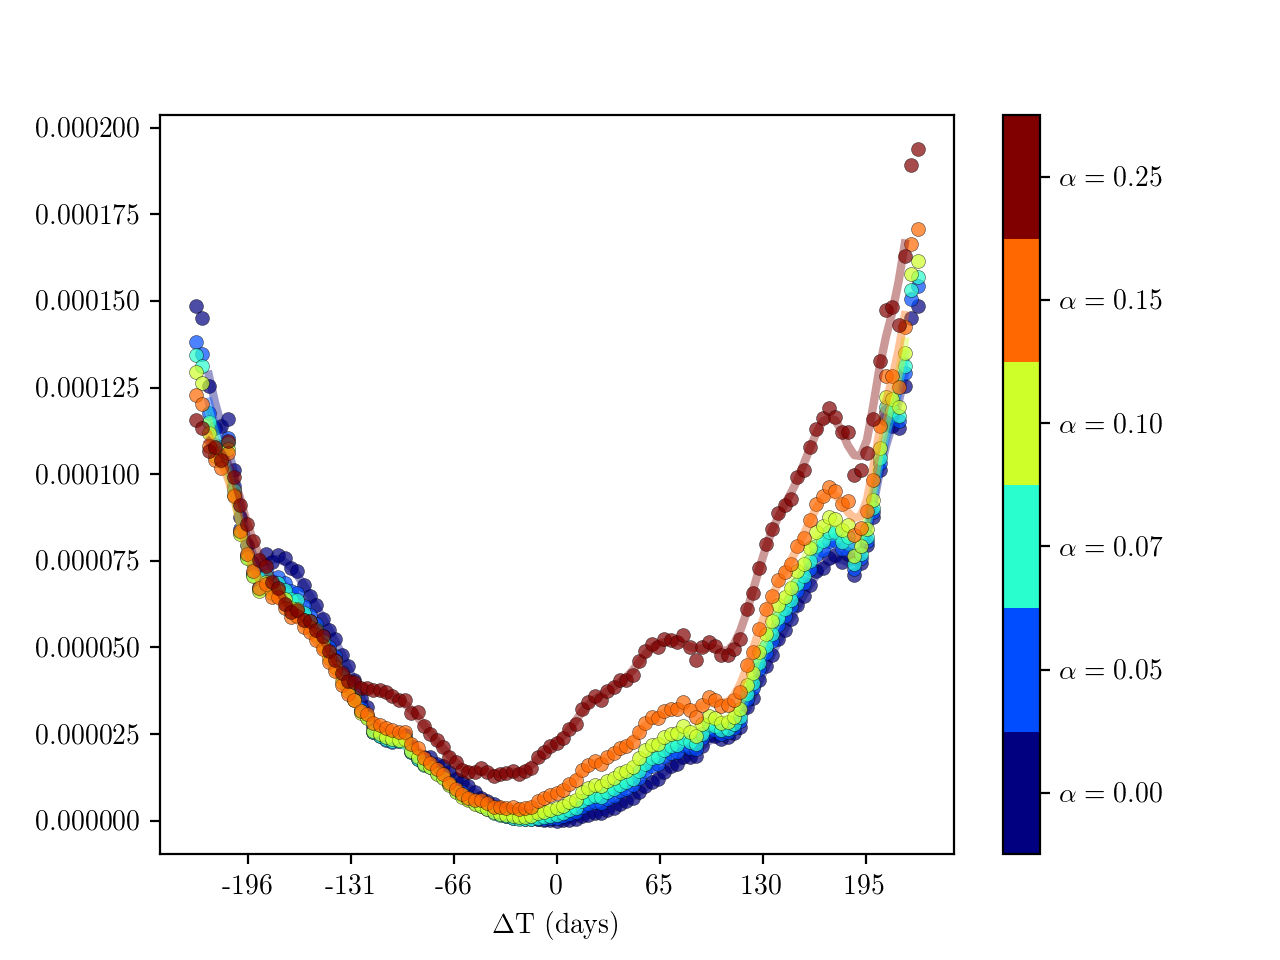
\includegraphics[height=0.32\textheight]{figs/dt_vs_err/better_at_past_G4D_9.png}\\
		($N=15$)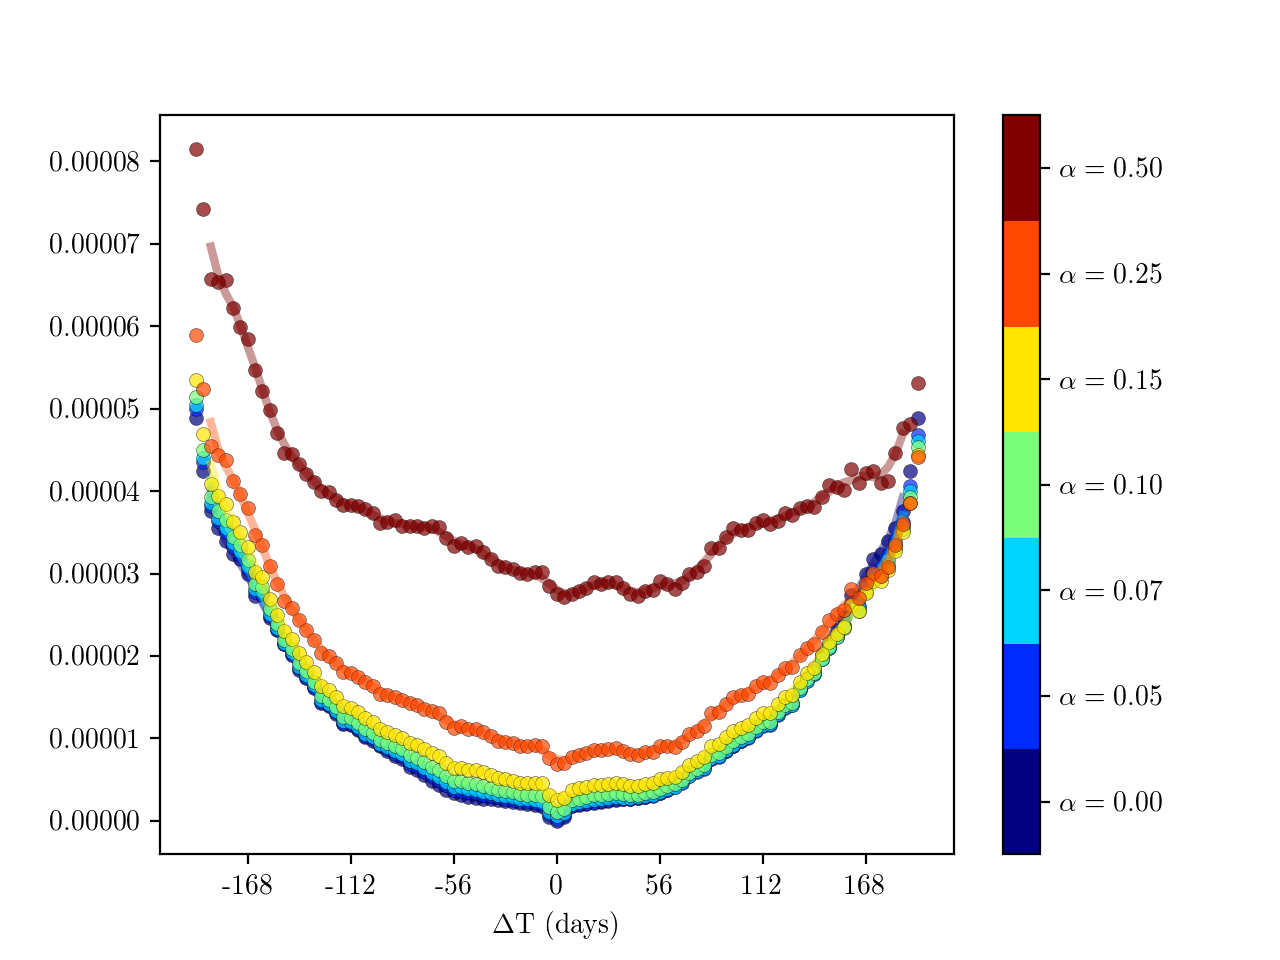
\includegraphics[height=0.32\textheight]{figs/dt_vs_err/balanced_G4D_15.png}\\
		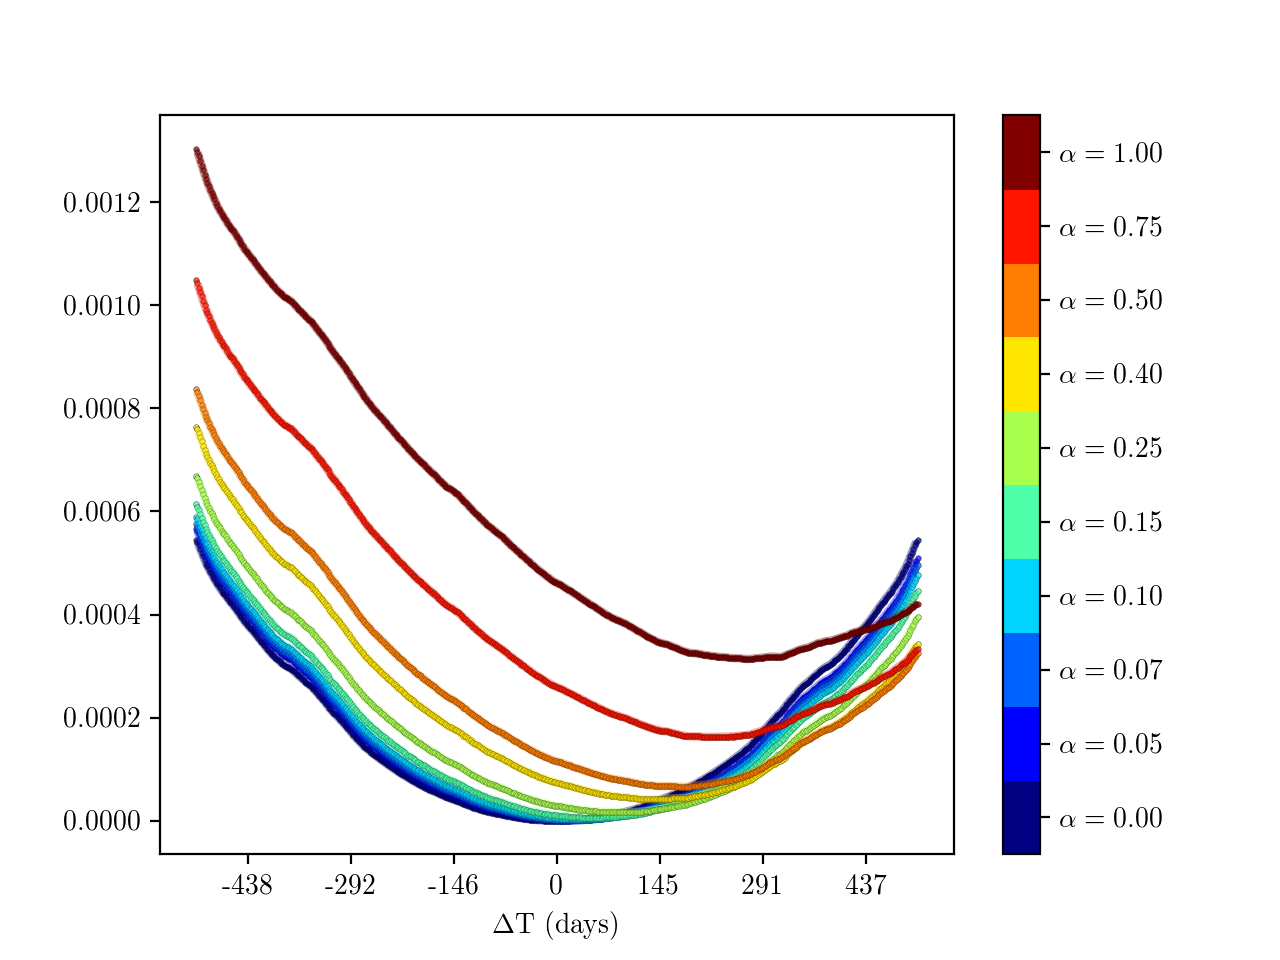
\includegraphics[height=0.32\textheight]{figs/dt_vs_err/G2D_30.png}~
		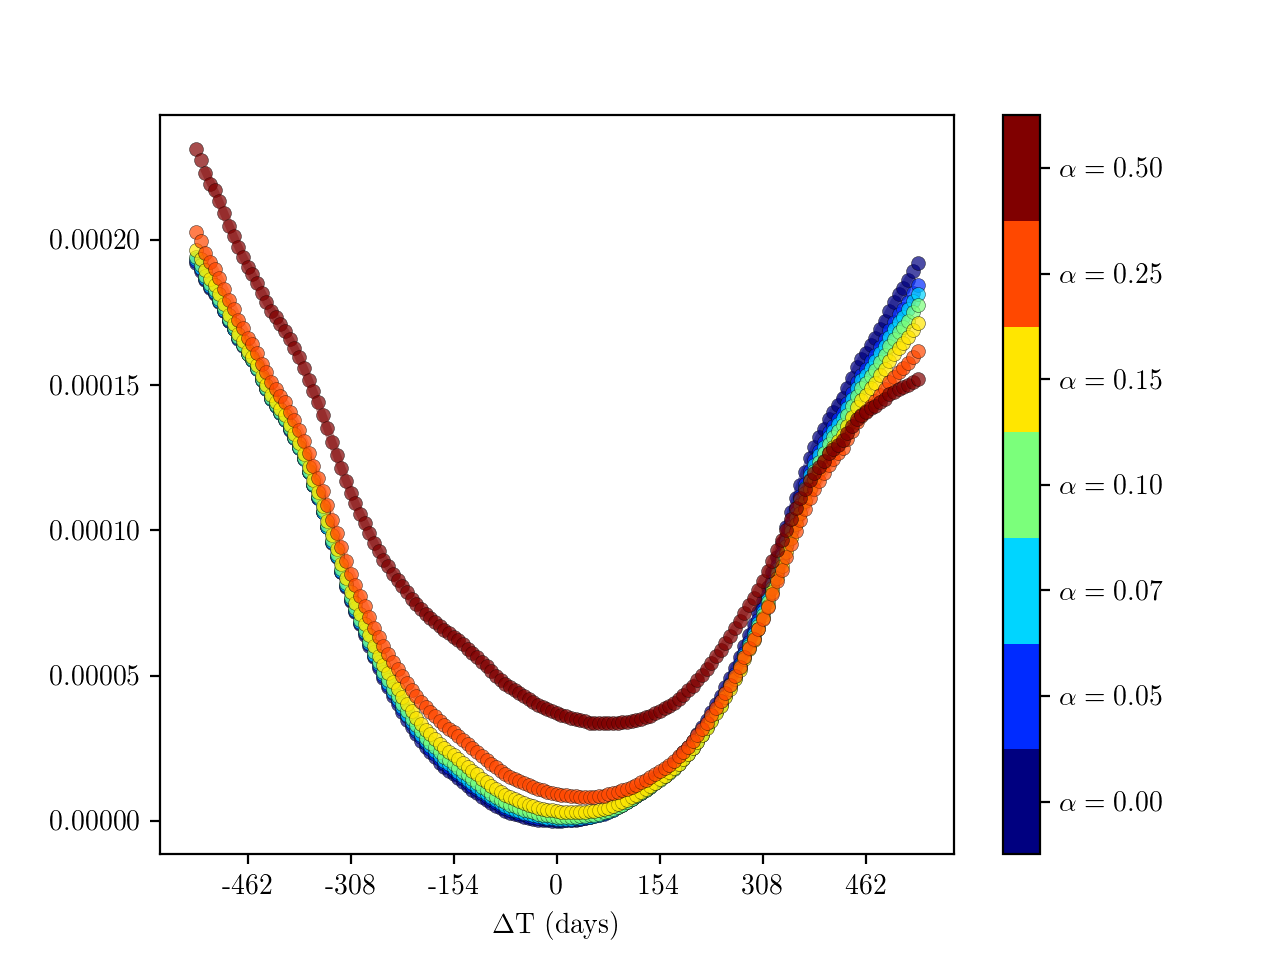
\includegraphics[height=0.32\textheight,width=0.5\linewidth]{figs/dt_vs_err/better_in_future_G1W_100.png}\\
		($N=30$)\hspace{2in}($N = 100$)
		\caption{\color{darkgray} Tradeoff between $\alpha$ and $\Delta T$. For small $N$, the curve shifts backwards in time. In the mid-range, $Q$ is better than $\Psi Q$, and for high $N$, the error is future shifted}
		\label{fig:nnodes_bias_dir}
	\end{figure}

	Here is my speculation about why this is the case: for small $N$, we are looking only at the very most popular subs, by activity. In these subs, the increased ``utility'' we're measuring really is just increased posting activity. But in really large communities that already receive a great deal of posts, having more posts makes the actual post quality go down: the biggest subreddits become famously riddled with reposts and are almost incredibly difficult to moderate, until almost nobody stays there for very long. The issue with our model is not algorithmic, but rather that our surrogate for utility points in the wrong direction after a certain point. Of course, for big $N$, there will also be quite a few smaller subreddits, so our mean squared error will be brought down by cases where increased activity actually increases the utility of a community.
	

	\subsection{Utilites are Only Helpful for Near Future}\label{sec:utilsnearfuture}
	
	We still have yet to mention the impact of the utility normalization on the error. In figure \ref{fig:normproblem}, we we are plotting the error against $\Delta T$, for utilities scaled by the ratio $r$ (Utilites which are by default normalized to 15), for two different temporal subgraphs. 
	
	\begin{figure}[h!]
		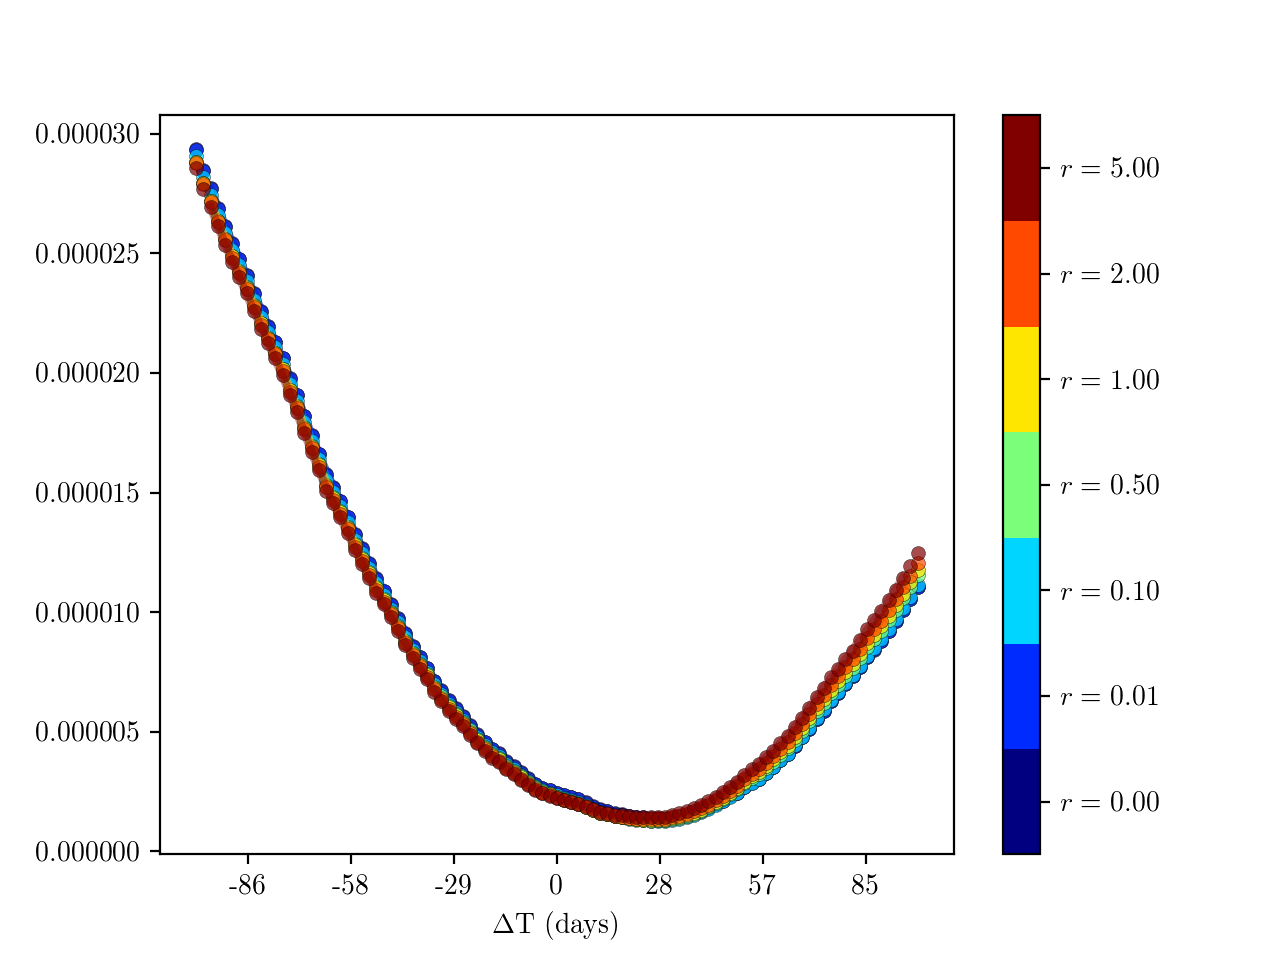
\includegraphics[width=0.5\linewidth]{figs/uscale/G2D30_a07_big.png}
		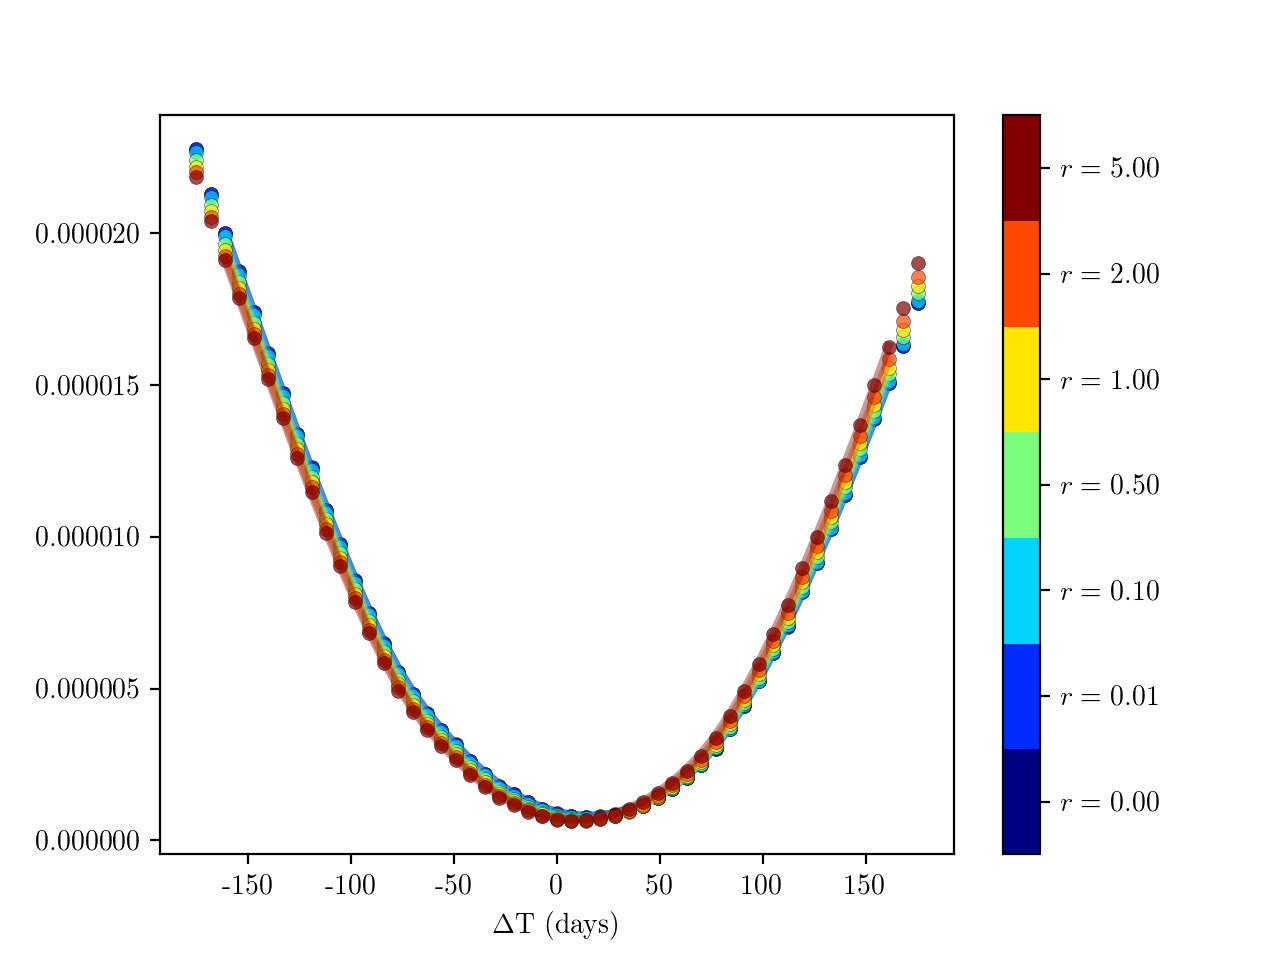
\includegraphics[width=0.5\linewidth]{figs/uscale/G1W100_a07_big.png}
		\caption{\color{darkgray} Big picture: with zero'd out utilities, seems to outperform the version that takes utility into account. left: $N = 30$, right: $N=100$. Both: $\alpha = 0.07$. Utilities are base scaled to a maximum of 15, and then multiplied by the factor $r$ (colorbar)}\label{fig:normproblem}
	\end{figure}

	The worrying bit is that the dark blue curve, in which we set all utilities to zero, seems to be more future-shifted than the ones in which we actually use utilities. Clearly, the curves are extremely close, at any rate. However, upon zooming in on timescales closer to zero, as in figure \ref{fig:resolvenorm}, we can see that adding utilities only makes predictions better, on the timescale of 25 days. This is true across values of $\alpha$, as shown in the figure.

	\begin{figure}
		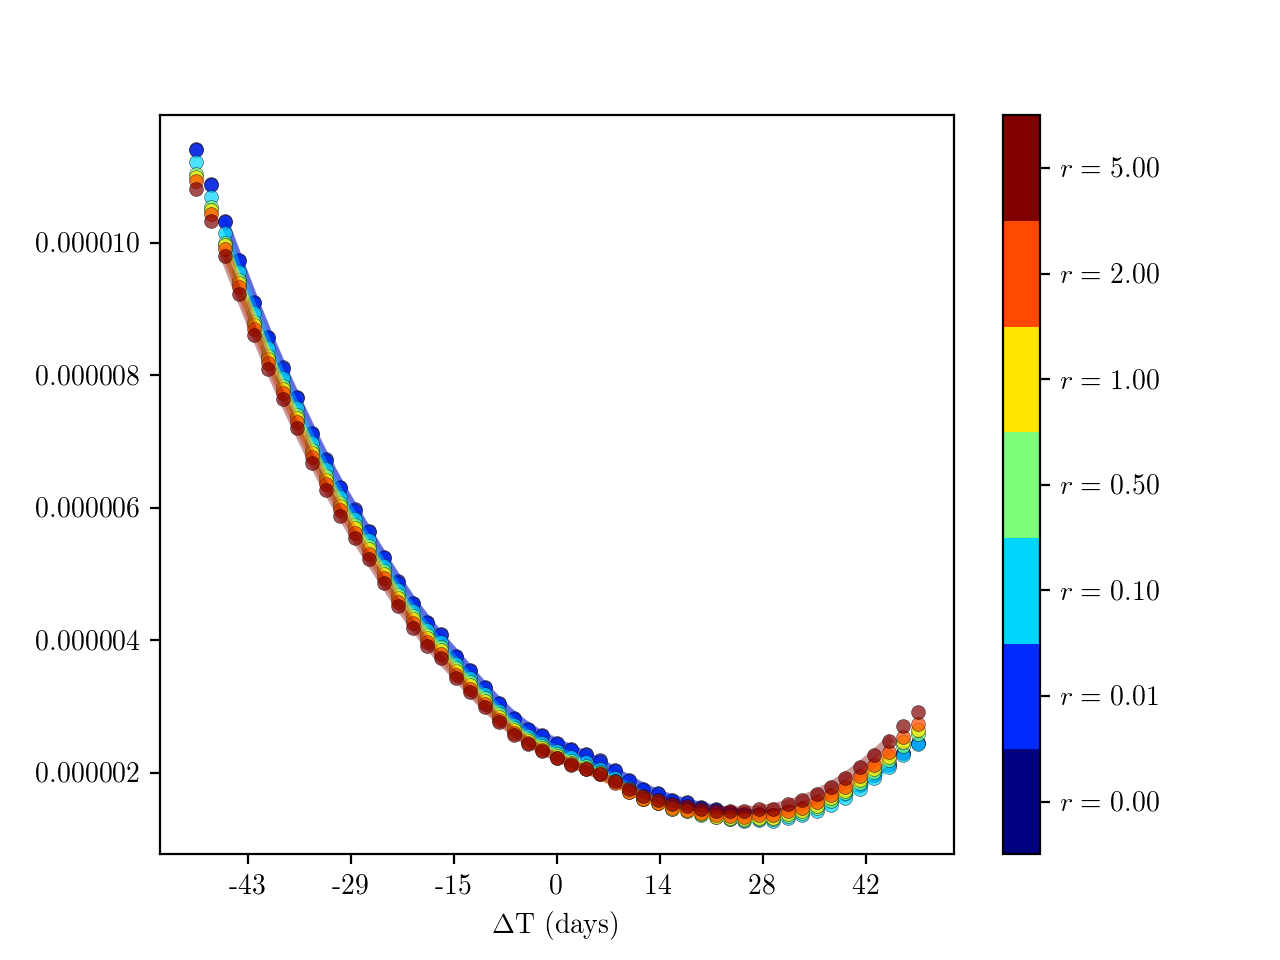
\includegraphics[width=0.5\linewidth]{figs/uscale/G2D30_a07.png}
		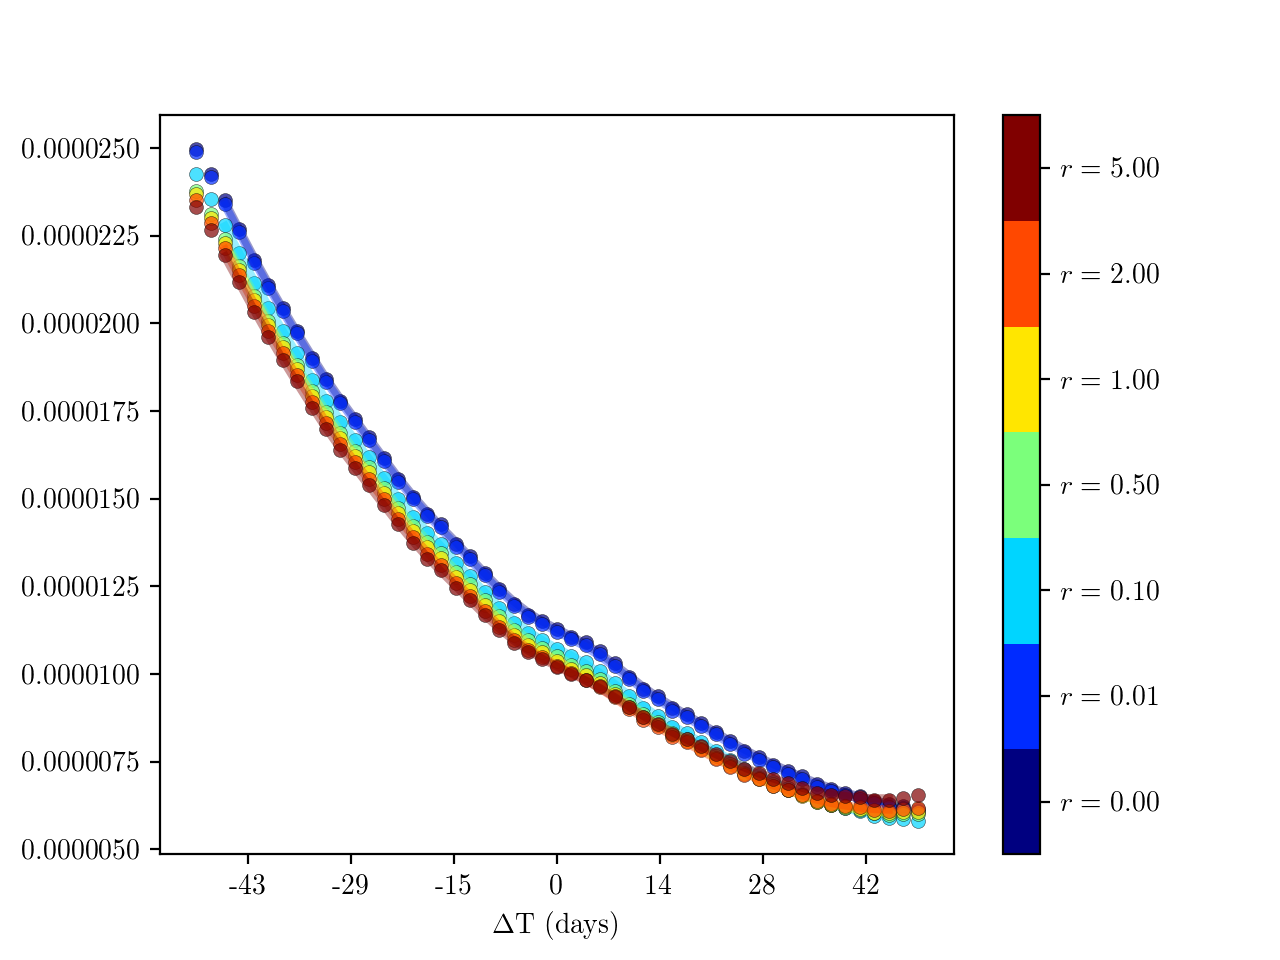
\includegraphics[width=0.5\linewidth]{figs/uscale/G2D30_a15.png}
		\caption{\color{darkgray} A zoomed in view of error for smaller positive values of $\Delta T$. left: $\alpha = 0.07$, right: $\alpha =0.15$. Both: $N = 30$. Utilities are base scaled to a maximum of 15, and then multiplied by the factor $r$ (colorbar)} \label{fig:resolvenorm}
	\end{figure}

	The interpretation here is that in the far future, we cannot really predict the utilities very well, and a simple coin flip model is a better way to predict the connectivity than taking this very flawed measure of utility into account. If, as we suspect, our measure of utility is upside-down for large subreddits, then this makes some sense: we can't predict the long-term dynamics because the information
	
	\section{Implementation}
	A large (often overlooked) chunk of the work for projects like these is software engineering, and in my view a third contribution of this project is a collection of utilities for scraping, storing, manipulating, and plotting doubly weighted temporal graphs. I want to quickly use some space to provide a quick overview, because it's actually rather reusable. It is available at \url{https://github.com/orichardson/util-graph-dynamics}. 
	
	\begin{itemize}
		\item \textbf{Experimental Utilities [\texttt{experimental.py}].} A lot of code for calculating different kinds of regressions and heatmaps on temporal graphs. Wrappers for discrete choice functions so that they behave like \texttt{scikit learn} regressors, and can therefore be re-used by built-in sklearn gridsearch, etc. Finally, a class called \texttt{rsltdict}, whose keys are frozen parameter dictionaries, and can be queried with keywords and constraints to quickly find results for certain parameters.
		
		\item \textbf{Reddit Scraping Code [\texttt{reddit\_graph\_builders.py}].}~ Code to build these temporal graphs from \texttt{pushshift.io} data, collecting any node or edge data, query the Reddit API to retrieve more recent karma information, and efficiently do batches under certain conditions. (It also has a compact console progress bar)
		
		\item \textbf{Data Structures [\texttt{temporal.py}].} A python class with operations for for adding, convolving, saving, loading, and building weight tensors from, temporal graphs.
		
		
		\item \textbf{Choice Transformer Construction [\texttt{choice.py}].} Perhaps less generally useful but contains things like interpolation, faster algorithmic implementations of the transformers defined in section \ref{sec:transformer}, logit modes, and column normalization.
		
		\item \textbf{Plotting for Discrete Graphs [\texttt{plotting.py}].} Three plotting functions built on top of \texttt{matplotlib}, which build \LaTeX rendered error plots, temporal animations, and heatmaps with date formatting, color bars, and automatically selects a subset of the information to display if too much is requested at once. They directly take temporal graphs objects without requiring explicit extraction of the relevant information.
	\end{itemize}

	
	\section{Limitations and Future Work}
	
	\subsection{Better Utility Approximation}
	The primary issue with the current framework, as mentioned in sections \ref{sec:futurebias} and \ref{sec:utilsnearfuture}, is the way we are calculating utilities. Fortunately, it should be quite easy to swap out code that does something else, in this framework. However, anything else is likely to be slower, as it cannot be done through an aggregated \texttt{pushshift.io} query. For instance, aggregating the karma submissions is straightforward to do, but difficult to do fast for arbitrary time winndows, since \texttt{pushshift.io} does not keep any up-to-date information. Another useful variable to consider while crafting a synthetic utility measure, is the number of unique posters in a sub.
	
		
	\subsection{Better Exploration of Neighborhood Distribution}
	
	There are many opportunities explore alternate discrete choice models more thouroughly. While we propose several, we stuck with just one for the majority of the simulations because it was much faster to simulate, and seemed to have similar or better performance. However, sampling neighborhoods is also a well-studied problem, and we can use something like \texttt{node2vec} \cite{grover2016node2vec} random walks is more likely to give us sampled neighborhoods which reveal graph structure, than our own custom, easy to integrate formulas.
	
	
	\subsection{More Principled Ways of Generalizing Parameters across Temporal Subgraphs}
	The way that I conducted the majority of this project was to simply select a few subgraphs that I had downloaded (they take a while to construct) and play around with visualizing things until I could understand what was going on, more-or-less. For parameters like the mixture coefficient $\alpha$, offset $\Delta T$, and the utility scaling $r$, I was able to automate grid searches over parameter spaces, resulting in satisfying plots like the ones shown. However, over variables like the number of node $N$ (which is confounded with node popularity due to the way I selected graphs), there was no good way to do this without worrying about the variables having confounding dependencies.
	
	Future work along these lines might aim to improve the selection of graphs by expanding to less popular subs in different ways. Perhaps it even makes sense to use the neighborhood sampling techniques one might implement from \texttt{node2vec} here too.
	
	\subsection{Related Experiments}
	\subsubsection{Utility Prediction}
	Rather than predicting $Q$, we could also predict $U$, which would be easier for networks and SVMs to handle, as there are fewer outputs that need to be learned. This is interesting, as it corresponds to the question of how the utilities change in the first place 
	
	\subsubsection{Better Predictors: Neural or Structured} By engineering better ML baselines systems, ether by exposing better features (we definitely want some shared weights in the predictor; one possibility is exposing only the relevant rows and columns and training a single regression which we permute to get all the entries of the output matrix), or by throwing a lot more data and better network architecture at the problem, we can probably do a lot better at this task.  
	
	\subsection{Individual Variation}
	In our formulation, we have assumed that there is a static utility function $U$ on the vertices of the graph, governing choice. For many applications, this one included, some people will prefer some places to others. In many ways, this is one of the distinguishing features that causes there to be places at all. The utility data we have gathered is not from an individual, but rather the aggregate ``will of the people''. However, it is well-known that aggregate wills are not particularly agentive (e.g., the Condorcet paradox), and in general, we get another mixture paramter, for a deeper mixed logit model, rather than altered utilities for our current one. 
	
	One interesting direction might be to model this more carefully, and try to discern the nature and number of archetypes needed to better approximate the dynamic utilities of the graphs.

%	\section{Conclusions}
%	
%	We have 

	
	\printbibliography
	
	\appendix

	
	
%	\section{Motivation}

%	
%	Outside of this class, I'm looking to formalize the theory of rational preference change as a fused combined RL / IRL (inverse reinfocement learning) problem. However, this would be a much better theory if it were empirically validated --- I propose to use reddit as a source of purely frivolous preference data. The karma (upvote/downvote) associated with each post or comment can be thought of as a proxy for the collective preferences of the subset of the community who read and cared about the comment. This system was designed purely to sort through posts, but in doing so, it has exposed annotations of the ``good''-ness of large amounts of text and images in context.
%	
%	
%	\section{Empirical Study}
%	
%	\subsection{Research Questions}
%	Ultimately, we would like to know why people actually change their preferences: whether it is done in a consistent manner, and whether this can be considered rational. To this end, we will discuss the evolution of both individual users and communities' preferences over time. 
%stable
%	
%	Below is a list of relevant questions that I expect to be able to shed some light on. I am aware that I will not have time for all of them.
%	\begin{enumerate}
%		\item Is there a scale symmetry between individuals and communities --- do the mechanisms by which they appear to change differ substantially beyond the time-scales and numbers of total interactions?
%		
%		\item To what degree do memes bleed from one community to another?
%		\item What determines the lifetime of a meme, beyond noise? Are humans any good at it? We can use \texttt{r/MemeEconomy} to get data on humans predicting meme longevity, plus historical data about how good individuals have been in the past.
%		
%		\item What kinds of posts cause a sub to grow or shrink? 
%		
%		\item How do community preferences evolve over time, as measured directly by statistics of the content, and as measured by the topology of the interactions between users and communities?
%	\end{enumerate}
%
%	
%
%
%
%	
%
%	\section{Outline of Experiments}
%	Reddit can be thought of as a graph data set in a number of different ways; applying the numerical methods we covered in class may reveal different kinds of preference data.
%
%	\subsection{Content Representation $\mathcal T$}
%		
%	First, because I do not want to be doing complex NLP myself for the purposes of this project, I will need to import an existing space $\mathcal T$, and embedding $\eta: \Gamma \times \mathrm{Text} \times \mathrm{Image} \to \mathcal T$, where $\Gamma$ is a context space, equipped with an applicative structure $\mathrm{Text} \times \Gamma \to \Gamma$. This will allow me to embed posts, captions, and images, into a single space for convenience, and be a control for the network analyses that follow.
%	
%	\subsection{Subreddit Drift}
%	The nodes are subs, and there are edges between them corresponding to top-level comments referencing a (different sub). These edges each have a weight and time associated with them (corresponding to the karma and date of thIfe comment), so we can apply the methods presented in class for analyzing temporal graphs.
%	
%	Temporal motifs here correspond to interactions between subs. Even simply by partitioning the graph into time windows, we can see how the subs move about in the induced preference space that we would expect from a node embedding. Moreover, these data can be compared from the data obtained from motion of the average post within the content space $\mathcal T$.
%	
%	Clustering will almost certainly reveal closely linked communities (probably even often explicitly, as many subreddits link to one another in side bars, and the graph generated by these edges can be compared to the one generated temporally through comment links). More importantly for my purposes, the clustering will likely change as time goes on -- when it changes, we would like to identify either graphical motifs or pieces of content space which tend to proceed shifts. Our hope is that the correlations and anti-correlations between content-space and co-reference space will shine some light on why these effects occur.
%	
%	\subsection{User Drift}
%	The nodes are users, and there is an edge $i \to j$ when user $j$ comments on a post or comment made by $i$. These links also have both weights and times associated with them, for the same reasons. This is the structure which most directly addresses the question at hand, because users themselves are definitely agents, and the ways in which they interact with the site reflect their evolving preferences. However, because of small amounts of data for individual users, we expect that it will be difficult to identify a causal picture of this.
%	
%	\subsection{The Reddit Hierarchy and Flow}
%	
%	Comments, posts, and subs are all nodes, and edges between them are sub-post relations: each post has a parent-edge to its sub, and comments have edges to their posts or parent comments. Again, all of these entities have weights (karma / subscribers) and times. 
%	
%	In this case, we expect role labeling to recover which of the nodes are actually comments, posts and subs; this is a sanity check, and shows that the way that people interact with these elements 
%	
%	In some sense, this is the most boring network interpretation of the site, because it is the one shown to users and developers, and is simply an abstraction tree presented to the world. However, if we look at it as a temporally evolving tree, and we additionally consider it as the co-domain of the number of subscribers / karma, we may be able to discover more interesting structure. In particular, if attention is flowing through the graph based on this topology, we might ask if there is a stationary distribution on $\eta$-equivalence classes of nodes (perhaps community dependent), and ask how this stationary distribution shifts over time.
%
%	
%	\section{Numerical Methods: Possibilities for Theoretical Advancement}
%	
%	I suspect that treating groups of users (potentially even large users) as a single users with well-defined preferences as users themselves, will result in very similar analyses. For this reason, we may want to understand graphs not in terms of their small-scale motifs, but rather scale-invariant ones. If I have additional time / energy, or this falls out of the project naturally, then I would like to formalize the effect of collapsing larger groups of nodes into a single one on motif analysis, and design one that is robust to this kind of . This is particularly important from the point of view of tropical geometry, in which collapsed vertices correspond to degenerate polynomials, which mostly behave in exactly the same way as every one of the graphs that they could represent.
	
\end{document}